\documentclass{report}

% ---------- Encoding & Layout ----------
\PassOptionsToPackage{table,dvipsnames}{xcolor} % add any colorsets you need
\usepackage{xcolor}
\usepackage[T1]{fontenc}
\usepackage[utf8]{inputenc}
\usepackage[a4paper, total={6in, 8in}]{geometry}

% ---------- Math / Fonts ----------
\usepackage{amsmath}
\usepackage{amsfonts}

% ---------- Graphics ----------
\usepackage{graphicx}
\graphicspath{{./images/}}
\usepackage{subfig}
\usepackage{float}
\usepackage[final]{pdfpages}
\usepackage{pdflscape}
\usepackage{rotating}


\definecolor{darkGrey}{gray}{0.3}

% ---------- Colors (define before hyperref) ----------
% \usepackage{xcolor}
% Colors for tables
% \usepackage[table]{xcolor} % or: \usepackage{colortbl}
\definecolor{darkGrey}{RGB}{77,77,77} % adjust to taste
\definecolor{deepblue}{rgb}{0,0,0.5}
\definecolor{deepred}{rgb}{0.6,0,0}
\definecolor{deepgreen}{rgb}{0,0.5,0}
\definecolor{maroon}{rgb}{0.5,0,0}
\definecolor{darkgreen}{rgb}{0,0.5,0}
\definecolor{backcolour}{rgb}{0.95,0.95,0.92}
\definecolor{codegreen}{rgb}{0,0.6,0}

% ---------- Listings (use this instead of minted to avoid --shell-escape) ----------
\usepackage{listings}
\lstdefinestyle{myStyle}{
  backgroundcolor=\color{backcolour},
  commentstyle=\color{codegreen},
  basicstyle=\ttfamily\small,
  breakatwhitespace=false,
  breaklines=true,
  keepspaces=true,
  numbers=left,
  numbersep=5pt,
  showspaces=false,
  showstringspaces=false,
  showtabs=false,
  tabsize=2
}
\lstset{style=myStyle}

\usepackage{listingsutf8}   % UTF-8 support for listings
\usepackage{inconsolata}    % nicer monospaced font (optional)
\usepackage{upquote}        % straight quotes in verbatim/listings

\lstset{
  inputencoding=utf8,
  basicstyle=\ttfamily\small,
  columns=fullflexible,
  keepspaces=true,
  breaklines=true,
  showstringspaces=false,
  % Map common UTF-8 characters to TeX equivalents:
  literate=
    {–}{{--}}1  % en dash
    {—}{{---}}1 % em dash
    {…}{{\ldots}}1
    {’}{{'}}1
    {“}{{``}}1
    {”}{{''}}1
    {−}{{-}}1   % Unicode minus
}


% XML language for listings
\lstdefinelanguage{XML}{
  basicstyle=\ttfamily,
  morestring=[s]{"}{"},
  morecomment=[s]{?}{?},
  morecomment=[s]{!--}{--},
  commentstyle=\color{darkgreen},
  moredelim=[s][\color{black}]{>}{<},
  moredelim=[s][\color{red}]{\ }{=},
  stringstyle=\color{blue},
  identifierstyle=\color{maroon}
}

% Optional Python styling macro (no undefined \ttb/\ttm)
\newcommand\pythonstyle{\lstset{
  language=Python,
  keywordstyle=\bfseries\color{deepblue},
  emph={MyClass,__init__,def,if,else,try,except,while},
  emphstyle=\bfseries\color{deepred},
  stringstyle=\color{deepgreen},
  frame=tb,
  showstringspaces=false
}}

% ---------- Other utilities ----------
\usepackage{comment}
\usepackage{fancyhdr}
\usepackage{blindtext}
\usepackage{lastpage}
\usepackage{mdframed}

% ---------- Hyperref (load last) ----------
\usepackage{hyperref}
\hypersetup{
  colorlinks=true,
  linkcolor=blue,
  citecolor=blue!50!black,
  urlcolor=blue!80!black,
  pdftitle={Overleaf Example},
  pdfpagemode=FullScreen
}

% ---------- Header / Footer ----------
\pagestyle{fancy}
\fancyhf{}
\rhead{\today}
\lhead{%
  \IfFileExists{images/imap_logo.png}{
\includegraphics[width=3cm]{images/imap_logo.png}}{\fbox{imap\_logo.png}}%
  \hspace{1cm} \bfseries \Large IDEX Algorithms Template
}
\rfoot{%
  \IfFileExists{images/lasp_logo.png}{
\includegraphics[width=5cm]{images/lasp_logo.png}}{\fbox{lasp\_logo.png}}%
}
\fancyfoot[L]{Page \thepage\ of \pageref{LastPage}}

\setcounter{chapter}{-1}

\begin{document}

\begin{titlepage}
  \centering
  \vfill
  {\bfseries\Huge IDEX Algorithms Template\\
  \vskip2cm
  \Large Draft 8\\
  \vskip5cm
  Ethan Ayari\\
  Jamey Szalay\\
  Mihály Horányi\\
  \vskip3.5cm}
  \vfill
  \IfFileExists{images/lasp_logo.png}{
\includegraphics[width=10cm]{lasp_logo.png}}{\fbox{lasp\_logo.png}}
  \quad
  \IfFileExists{images/imap_logo.png}{
\includegraphics[width=10cm]{imap_logo.png}}{\fbox{imap\_logo.png}}
  \vfill
\end{titlepage}

\tableofcontents

\chapter{SDC Prompts}\label{chap:chap1}

All of the information below was taken from the website:\\
\url{https://lasp.colorado.edu/galaxy/display/IMAP/IMAP+SDC+Software+Developer+Guide}.

In addition, \textbf{from the IMAP SOC CDRL List Applicable Algorithms} is defined in the following sequence:\\[0.5\baselineskip]
Level 0 -- Level 1A\\
Level 1A -- Level 1B\\
Level 1B -- Level 2\\
Data culling

\section{List of Acronyms}
\begin{itemize}
  \item AID: Application Identifier
  \item APID: Application Process Identifier
  \item CDRL: Contract Data Requirements List
  \item CCSDS: Consultative Committee for Space Data Systems
  \item CoDICE: Compact Dual Ion Composition Experiment
  \item DAB: Decontamination Actuator Board
  \item FPGA: Field Programmable Gate Array
  \item FSW: Flight Software
  \item HG: High Gain
  \item IDP: Interplanetary Dust Particle
  \item IDEX: Interstellar Dust Experiment
  \item IMAP: Interstellar Mapping and Acceleration Probe
  \item ISD: Interstellar Dust
  \item LG: Low Gain
  \item MG: Mid Gain
  \item MSPS: Mega samples per second
  \item PUI: Pickup ions
  \item SDC: Science Data Center
  \item SDMP: Science Data Management Plan
  \item SOC: Science Operations Center
  \item SWAPI: Solar Wind and Pickup Ions
  \item TOF: Time of Flight
\end{itemize}

\section{Definitions}
\textbf{Algorithm:} In this text, algorithm refers to a finite sequence of well-defined, computer-implementable instructions needed to generate one or more data products using lower-level data, calibration, and ancillary information.\\[0.5\baselineskip]
\textbf{Code:} Computer-executable instructions in a common programming language may be compiled (if needed) and executed to perform designated computations.\\[0.5\baselineskip]
\textbf{Pseudocode:} Simplified code used in preliminary code design and layout.

% \section{Preparation Information}
% (your commented content remains unchanged)

\section{Suggested Algorithm Document Content}
\begin{enumerate}
  \item Definitions of Terms
  \item Description of Overall Approach
  \item Background on Heritage Instruments (if applicable)
  \item Background on heritage processing implementations (if applicable)
  \item Instrument measurement approach and relationship between data collection, telemetry packets, and data products
  \item Overall processing flow, e.g. step-by-step process description/diagrams
  \item Identification of and detail pertaining to dependencies on S/C or other instrument's data
  \item Calibration Data and associated application, including recommended calibration file formats
  \item Mathematical description of algorithm steps
  \item Equations, constants, and coefficients for science calibrations
  \item Pseudocode
  \item Examples of in-flight calibration update incorporation
  \item Telemetry packet decomposition information (possibly part of SE-005)
  \item Spice kernels to map instrument into spacecraft coordinate frame
  \item Equations and coefficients for Temperature Conversions (possibly part of SE-005)
  \item Equations and coefficients for engineering conversions (possibly part of SE-005)
  \item Observation time basis
  \item Expected maintenance tasks (e.g. updating calibrations)
  \item Approach to Rejection, Culling, or Flagging of Suspect/Bad Data
  \item Expected Uncertainties / Uncertainty Analysis
  \item Data Validation Steps
  \item Recommended Testing Approaches
  \item Special considerations and unusual circumstances
\end{enumerate}

\chapter{Introduction}
\section{Document Purpose}
This document provides a description of the algorithms used to produce science data products from the IMAP Interstellar Dust Experiment (IDEX) instrument measurements. The data products are documented in the IMAP Science Data Management Plan (SDMP). This document includes a description of the data collection and data products, as well as details of the processing flow, algorithms, and data processing tasks.
\section{Scope}
The intended purpose of this information is to enable members of the IMAP Science Data Center (SDC) to implement, test, and validate executable software that will routinely produce designated data products during the science mission. For IMAP, Science Algorithm Documentation consists of the combination of documentation, instructions, specifications, and any available reference/prototype computer code needed to produce a science data product.
\section{Document Organization}
The first two chapters of the document provide a brief overview of what IDEX is and how it takes measurements. Chapter \ref{chap:chap3} Introduces the IDEX instrument characteristics and expected performance. 
Chapter \ref{chap:chap4} describes the details of the modes of operation: Booting Mode, Idle Mode, Science Mode, Transmit Mode, Safe Mode, Survival Mode and a Decontamination Mode.  
Chapter \ref{chap:chap5} describes the necessary steps to convert data between each of the levels along the pipeline. Detailed information on packets and software is made available in the Appendix.



\chapter{IDEX Instrument Description}
\label{chap:chap3}
\section{Overview}
The Interstellar Dust Experiment (IDEX) is a high-resolution impact ionization time-of-flight (TOF) mass spectrometer that provides the elemental composition and mass distributions of ISD and IDP particles. IDEX links the interstellar gas phase composition, as obtained with IMAP-Lo and through PUIs with CoDICE and SWAPI, with the makeup of ISD and IDP particles. 
\begin{figure}[H]
    \centering
    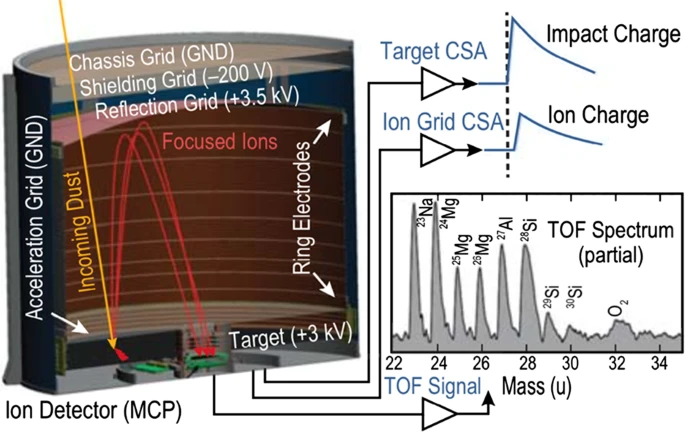
\includegraphics[width=\linewidth]{images/overview.png}
    \caption{An outline of the IDEX instrument and principle of operation. The three types of signals produced (ion grid, target and time-of-flight) are labeled and depicted by their corresponding hardware.}
    \label{fig:overview}
\end{figure}

IDEX is based on the heritage of past flight and laboratory instruments. Its operation principle is based on the impact ionization process.

IDEX has two components, an electronics enclosure and a sensor head with a large effective target area ($600$ cm$^2)$. The IDEX mechanical design consists of a simple Al shell structure that provides support for the biased electrodes of the TOF ion mass analyzer and the grids over its aperture. The centrally-located ion detector and the front-end charge sensitive amplifier are integrated into the bottom of the instrument.

 Individual dust particles entering the instrument pass through a set of grid electrodes and impact the target (Figure \ref{fig:overview}). The target is biased at +3 kV to provide positive ion acceleration and the reflectron-type ion optics are used to generate TOF compositional mass spectra. The impact-generated negative charges are collected on the target. An electrostatic field, shaped by a set of biased rings and a curved grid electrode, provides spatial and temporal focusing of the accelerated ions onto the central detector.


Target cleanliness is of high importance to be maintained throughout the fabrication, integration and operation of IDEX. The primary concern is the condensation of volatiles on the target. The mitigate this risk, 
IDEX has a one-time deployable door and its in-flight operation allows for the regular (once per months) use of heaters to raise the target temperature to 120 C over 8 hours in order to release any possible condensible contaminants. 

 
\section{Sensor Head}
An overview of the sensor head is shown in Figure \ref{fig:sensor}.

\begin{figure}[H]
    \centering
    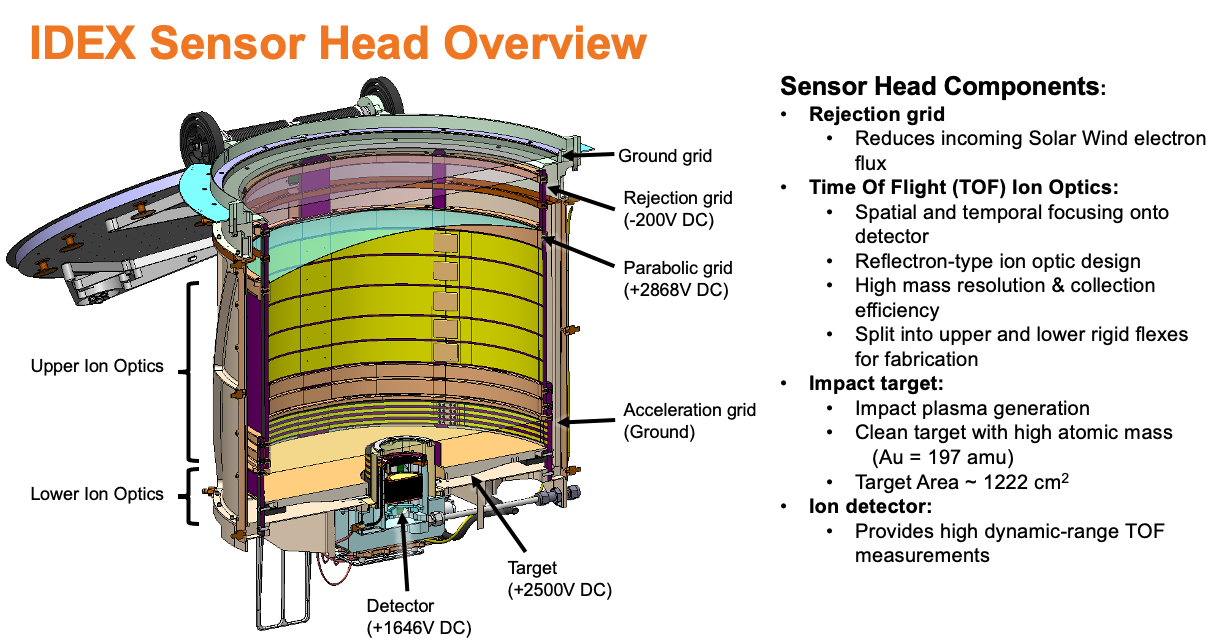
\includegraphics[width=\linewidth]{images/SensorHead.png}
    \caption{An outline of the IDEX instrument sensor head.}
    \label{fig:sensor}
\end{figure}

\section{Electronics}

The IDEX electronics leverage SUDA flight designs. The Decon/Actuator Board (DAB) is a new design that was added to control the door and decontamination heater.  The amplifier boards (CSA, Detector Buffer) were re-designed from the SUDA heritage instrument to meet the IDEX requirements for charge detection ranges. An overview of the IDEX electronics is depicted in Figure \ref{fig:elec}. 

\begin{figure}[H]
    \centering
    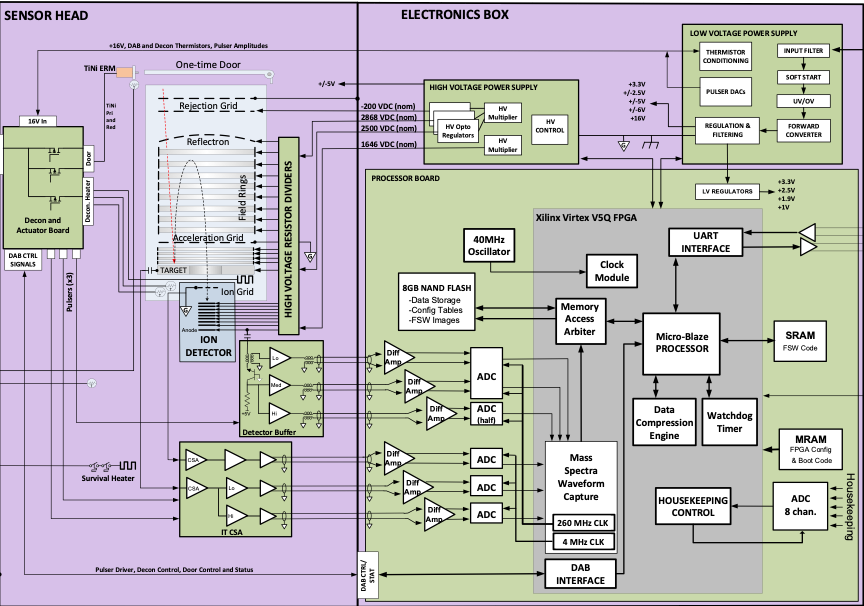
\includegraphics[width=\linewidth]{images/BlockDiagram.png}
    \caption{An outline of the IDEX instrument electronics system.}
    \label{fig:elec}
\end{figure}

%The electronics components relevant to the science data processing pipeline are the sensor head (excluding the Decon Actuator Board (DAB)) and the processor board. 

The 3 Time-of-Flight (TOF) gain stages, 2 Target CSA and 1 Ion grid CSA waveforms are the signals which the science data products are derived from. These constitute the packetized data accumulated in an 8 GB NAND flash and form the IDEX level 0 data product. 
\chapter{Nominal Operation}
\label{chap:chap4}
\section{Operating Modes}
IDEX has seven operating modes: off; boot;  and five nominal operations. A flow diagram showing how the instrument transitions through the various modes and a brief description of each is depicted in Figure \ref{fig:oper}. 

% DO WE HAVE A CHECKOUT MODE?
%CAPTURING WAVEFORMS TRIGGERED INTERNALLY?
%INJECTED PULSES?
% OR THOSE ARE NOT TO BE DISCUSSED IN THIS DOC?

\begin{figure}[H]
    \centering
    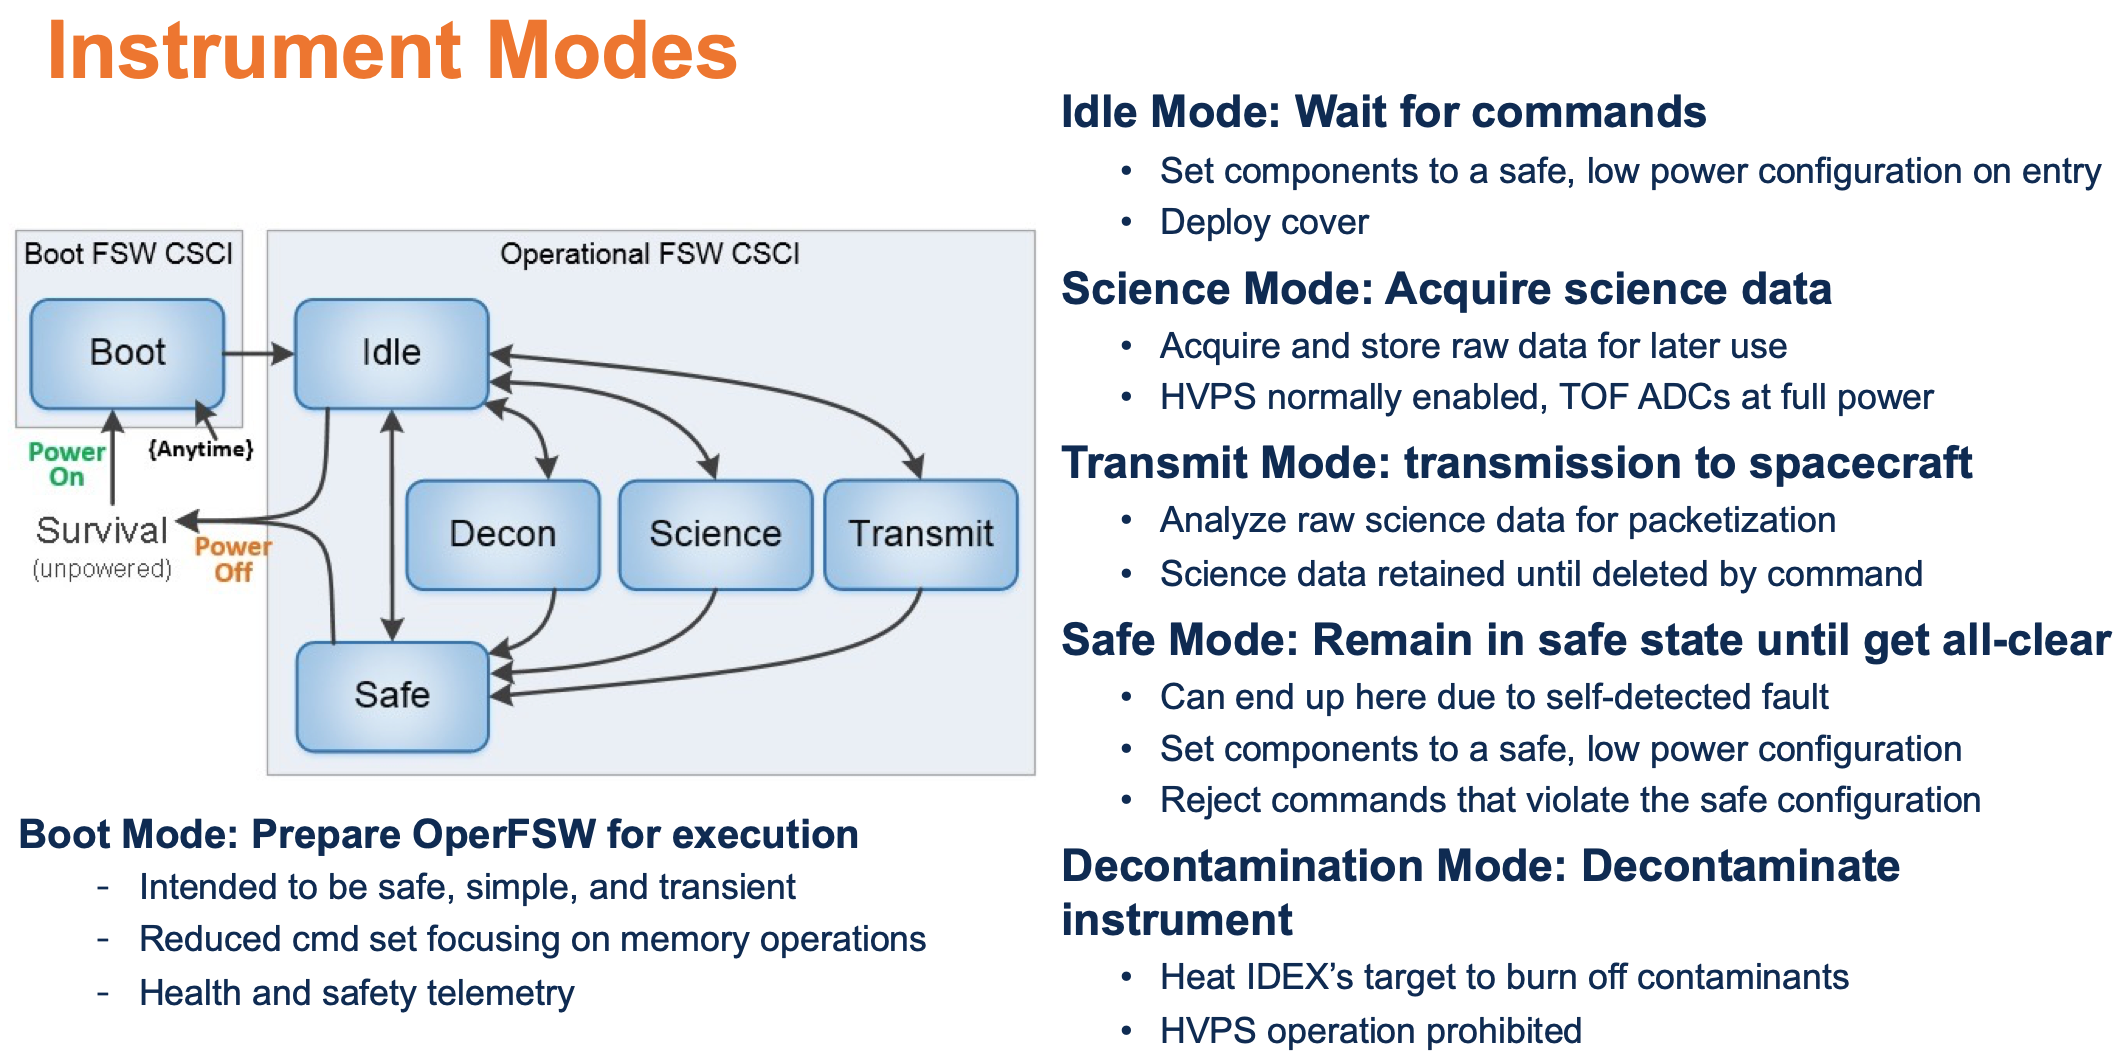
\includegraphics[width=\linewidth]{images/operation.png}
    \caption{An outline of the IDEX instrument operation modes.}
    \label{fig:oper}
\end{figure}


The \textbf{boot} mode is enabled when the instrument is powered on or any other time the operator indicates. In this mode, while FSW is performing a set of memory operations to prepare for execution, a health and safety telemetry packet is transmitted.

Following boot, the instrument enters its \textbf{idle} mode, %where the door is deployed 
and the instrument awaits commands. From here, the instrument may enter one of four possible operational modes, of which only two are relevant to the science data processing pipeline.

\subsection{Science Mode}
When the instrument enters the \textbf{science} mode, a memory buffer is continuously filled containing each of the 6 instrument signals. Since IDEX is an event-driven instrument, data is only packetized and transmitted when we have a dust impact, which we will refer to as an \textbf{event}. The instrument triggers based off of an event, sending the data stored in the memory buffer to the NAND flash.

The amount of data stored in a memory buffer depends on the sampling rate of the corresponding \textbf{analog-digital converter (ADC)}. The three time-of-flight gain stages are sampled at 260 MHz (high sampling rate). The two target gain stages and the ion grid, the ADCs are sampled at 4 MHz. Figure \ref{fig:pack} illustrates how data is packed for these two types of ADCs, as well as how much data is transmitted per event.

\begin{figure}[H]
    \centering
    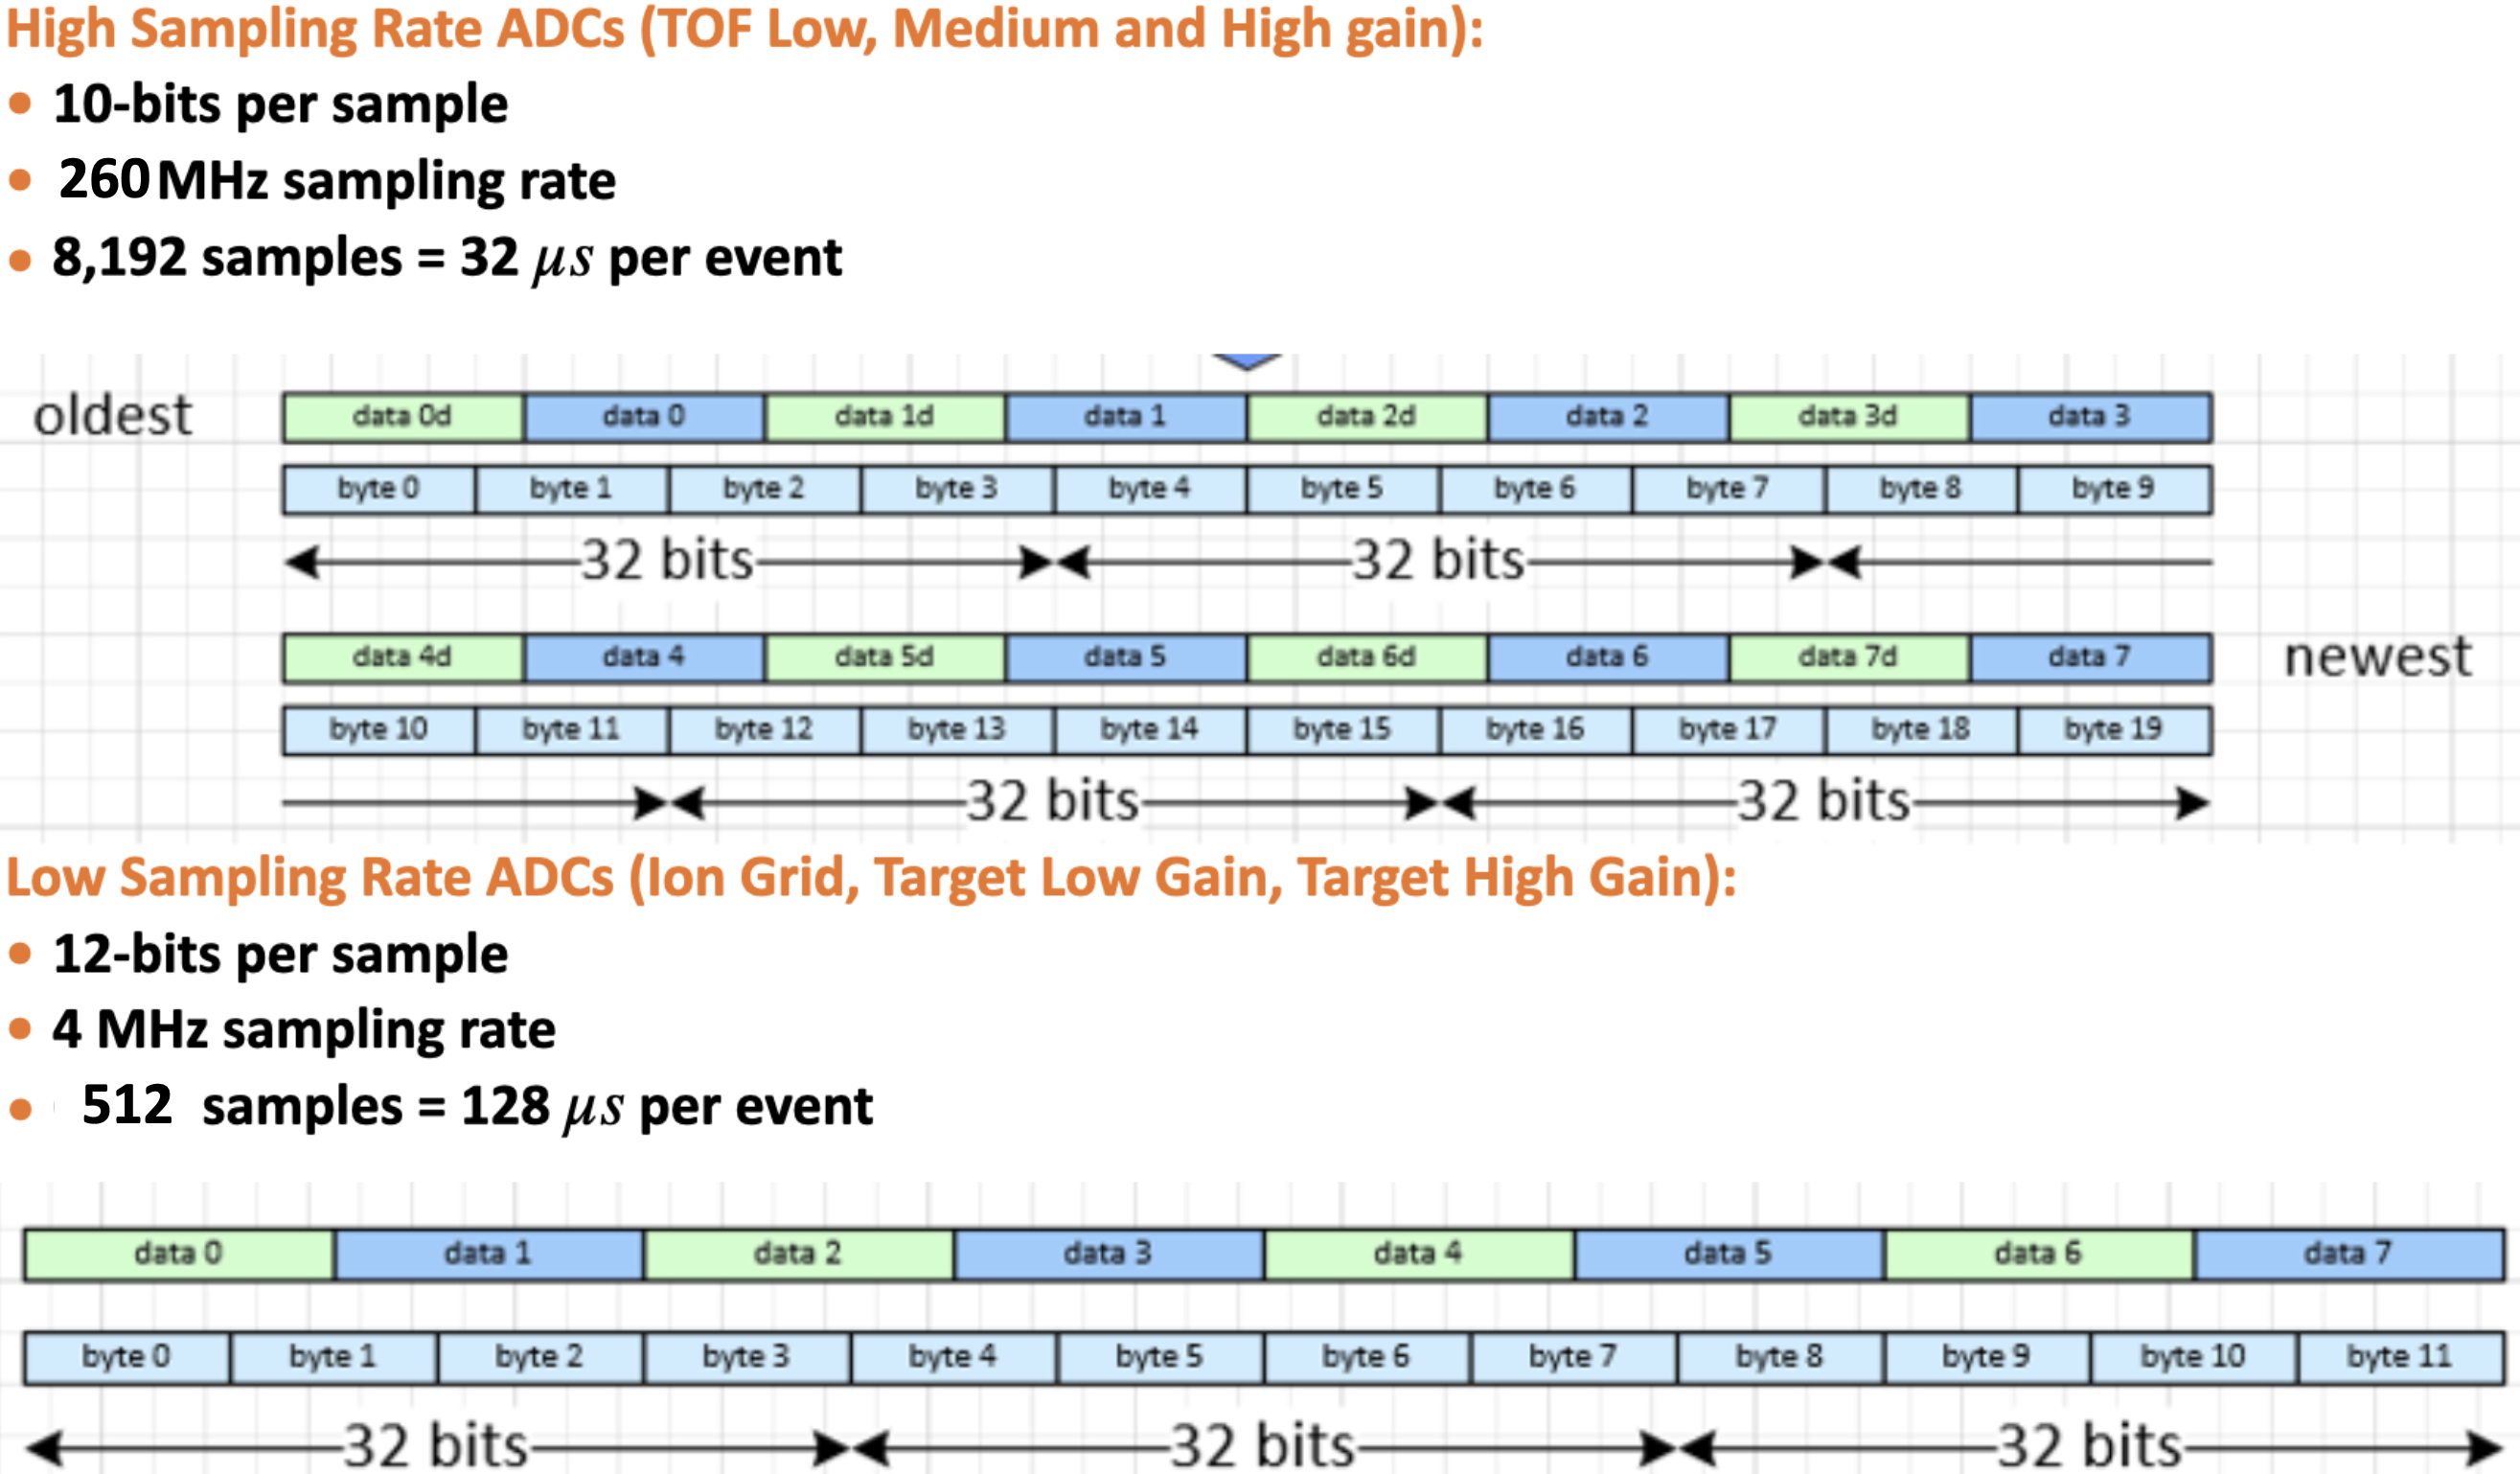
\includegraphics[width=\linewidth]{images/datapackaging.png}
    \caption{Diagram illustrating how data from the two different ADCs is packed in the NAND flash. Each event generates 88,064 bits of waveform data.}
    \label{fig:pack}
\end{figure}

\subsection{Transmit Mode}
Once the NAND flash has been populated with data from all 6 signals, it is ready for transmission. There are additional  post-trigger blocks based on the sampling rate of the corresponding ADCs, as pictured in Figure \ref{fig:adcf}.

\begin{figure}[H]
    \centering
    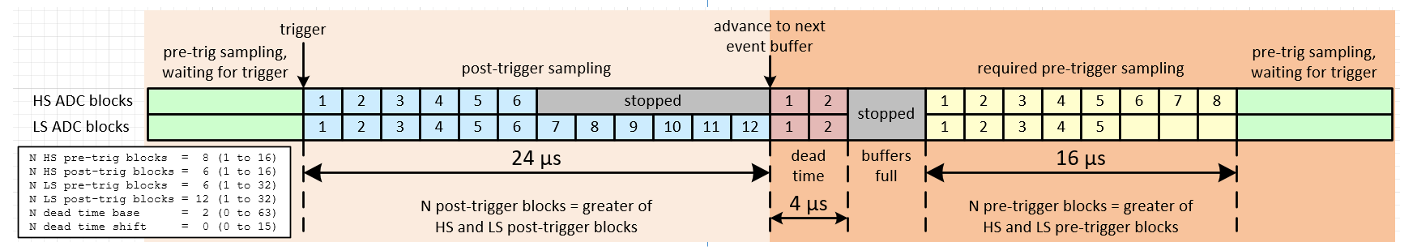
\includegraphics[width=\linewidth]{images/adcflow.png}
    \caption{Block diagram of the instrument timeline, based on high (HS) and low (LS) sampling rate ADCs.}
    \label{fig:adcf}
\end{figure}

Once the instrument triggers, there is a 4 $\mu$s dead time after the required post-trigger sampling has been completed. Hence,  at the very least, there will be a 4 $\mu$s gap between events. 

%This dead time is also optional if the instrument is expected to receive a high particle count.  NOT SURE WHAT THIS MEANS? CAN IDEX TURN OFF DEADTIME?

Transitions between instrument modes are driven by commands from the spacecraft. For the purposes of error detection and correction (EDAC), the 30 most recently executed commands and their associated timestamps are stored in the instrument log. This instrument log can be telemetered to the ground with the \textbf{DumpLog} command. These 30 commands include successful and failing command executions. However, if the command is so badly mangled that the FPGA or FSW is unable to recognize it as a command, then it does not get included in the log. %IS THERE A COUNTER FOR THESE ?

\subsection{Spacecraft Time Interface}

Each event is organized chronologically by the FPGA trigger time. For each event, the trigger time is stored in the event header. The event header is always specified by \textbf{SCI0TYPE=1} (see \ref{sci} for more details). This is given by a linear combination of the \textbf{SHFINE} and \textbf{SHCOARSE} variables. For each FPGA header, the \textbf{SHCOARSE} variable is a 16-bit unsigned integer that delineates the number of seconds since epoch (Midnight, January 1st, 2012)\textbf{SHFINE} variable indicates a number of 20 microsecond intervals in addition to the seconds since epoch.
Together, these time measurements establish when an event took place with respect to epoch. The formula to retrieve the epoch from the FPGA header is given by 

\begin{equation}
    \tau_{epoch} = SHFINE + 20*10^{-6}*SHCOARSE
\end{equation}

Additionally, the time axis for each of IDEX's 6 signals is derived from the sampling rate and the number of samples. The Ion Grid and two Target waveforms sample at 4 MHz, and the TOF sample at 130 MHz. The number of samples can then be multiplied by $3.846 \,[n s]$ and $246.15 \,[n s]$ for the time axis. \textbf{These samples are packed into blocks of 512 samples for the high sampling (HS) rate data and 8 for the low sampling (LS) rate data. The maximum amount of high-rate data is 16 blocks, which would be 8192 samples covering 31.5 us of time. The maximum amount of low-rate data is 64 blocks, which would be 512 samples covering 126.03 us of time.}
 
To line up the data, you need to line up the trigger point based on the settings for pre-trigger blocks and post-trigger blocks for the high-rate and low-rate data. For this, we turn to the \textbf{NBlocks/TXHDRBLOCKS} variable in each FPGA header. This variable is interpreted according to the map in figure~\ref{fig:nblocks}.

\begin{figure}[H]
    \centering
    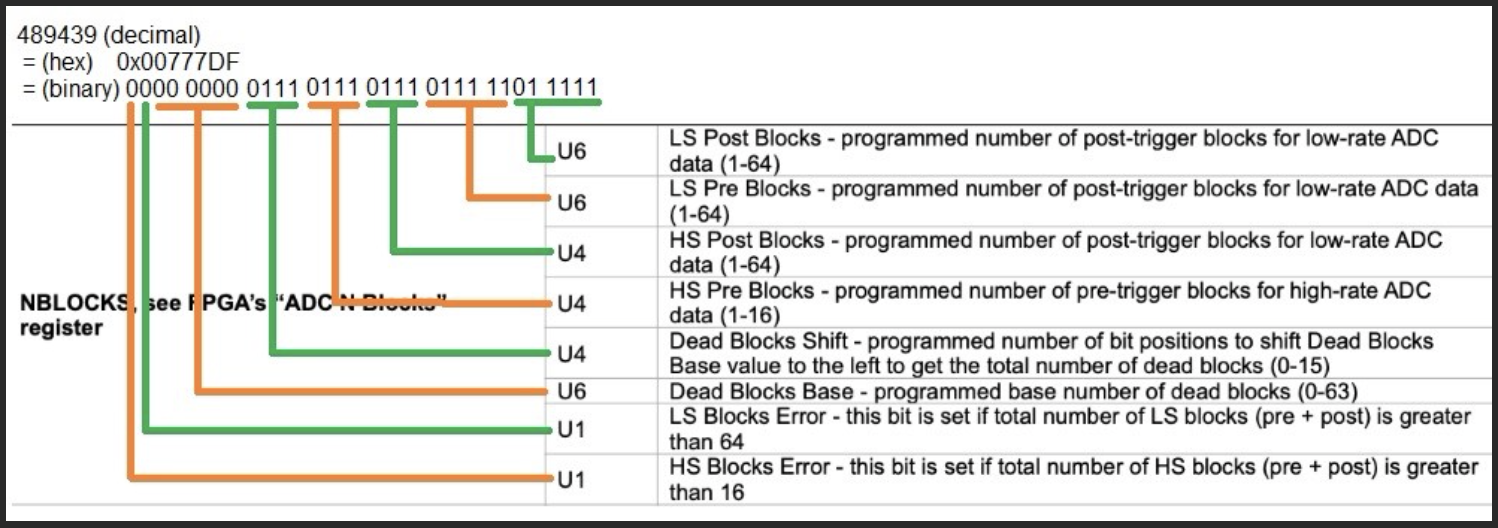
\includegraphics[width=\linewidth]{images/nblocks.png}
    \caption{Map showing how to decompose the \textbf{NBlocks} variable, provided by Greg Newcomb.}
    \label{fig:nblocks}
\end{figure}

The example shown is for a given integer value used during early integration and test, where the trigger was always in the middle of data acquisition (same number of pre and post trigger samples). Generally, this variable is a 32 digit binary string, which can be broken down as follows:

\begin{mdframed}[backgroundcolor=backcolour]{
 {\bf Digit 1} = 1 or 0 if there is an issue with the number of HS blocks. \\
 {\bf Digit 2} = 1 or 0 if there is an issue with the number of LS blocks. \\
 {\bf Digits 3-8} = Programmed base number of dead blocks: after post trigger sampling? \\
 {\bf Digits 9-12} = Dead blocks shift: Used with 3-8 to determine total number of dead blocks. \\
 {\bf Digits 13-16} = Number of high sampling pre-trigger blocks. \\
 {\bf Digits 17-20} = Number of high sampling post-trigger blocks. \\
 {\bf Digits 21-26} = Number of low sampling pre-trigger blocks. \\
 {\bf Digits 27-32} = Number of low sampling post-trigger blocks. \\
} \end{mdframed}

\section{Nominal Science Operations}
IDEX is an event-driven instrument, so data collection only takes place in the event of a trigger. Otherwise, when in science mode the instrument will continuously fill and delete the memory buffer. 



\section{Data Products}
The IDEX science data products pipeline takes raw instrument CCSDS packets (level 0 data) as inputs and goes through each stage of the mass spectrum calibration process to reveal the composition, target impact charge, and ion-grid charge of each measured dust particle (level 3 products). Each science data product level is delineated below in 
Table~\ref{fig:levels}.
\begin{table}[H]
    \centering
    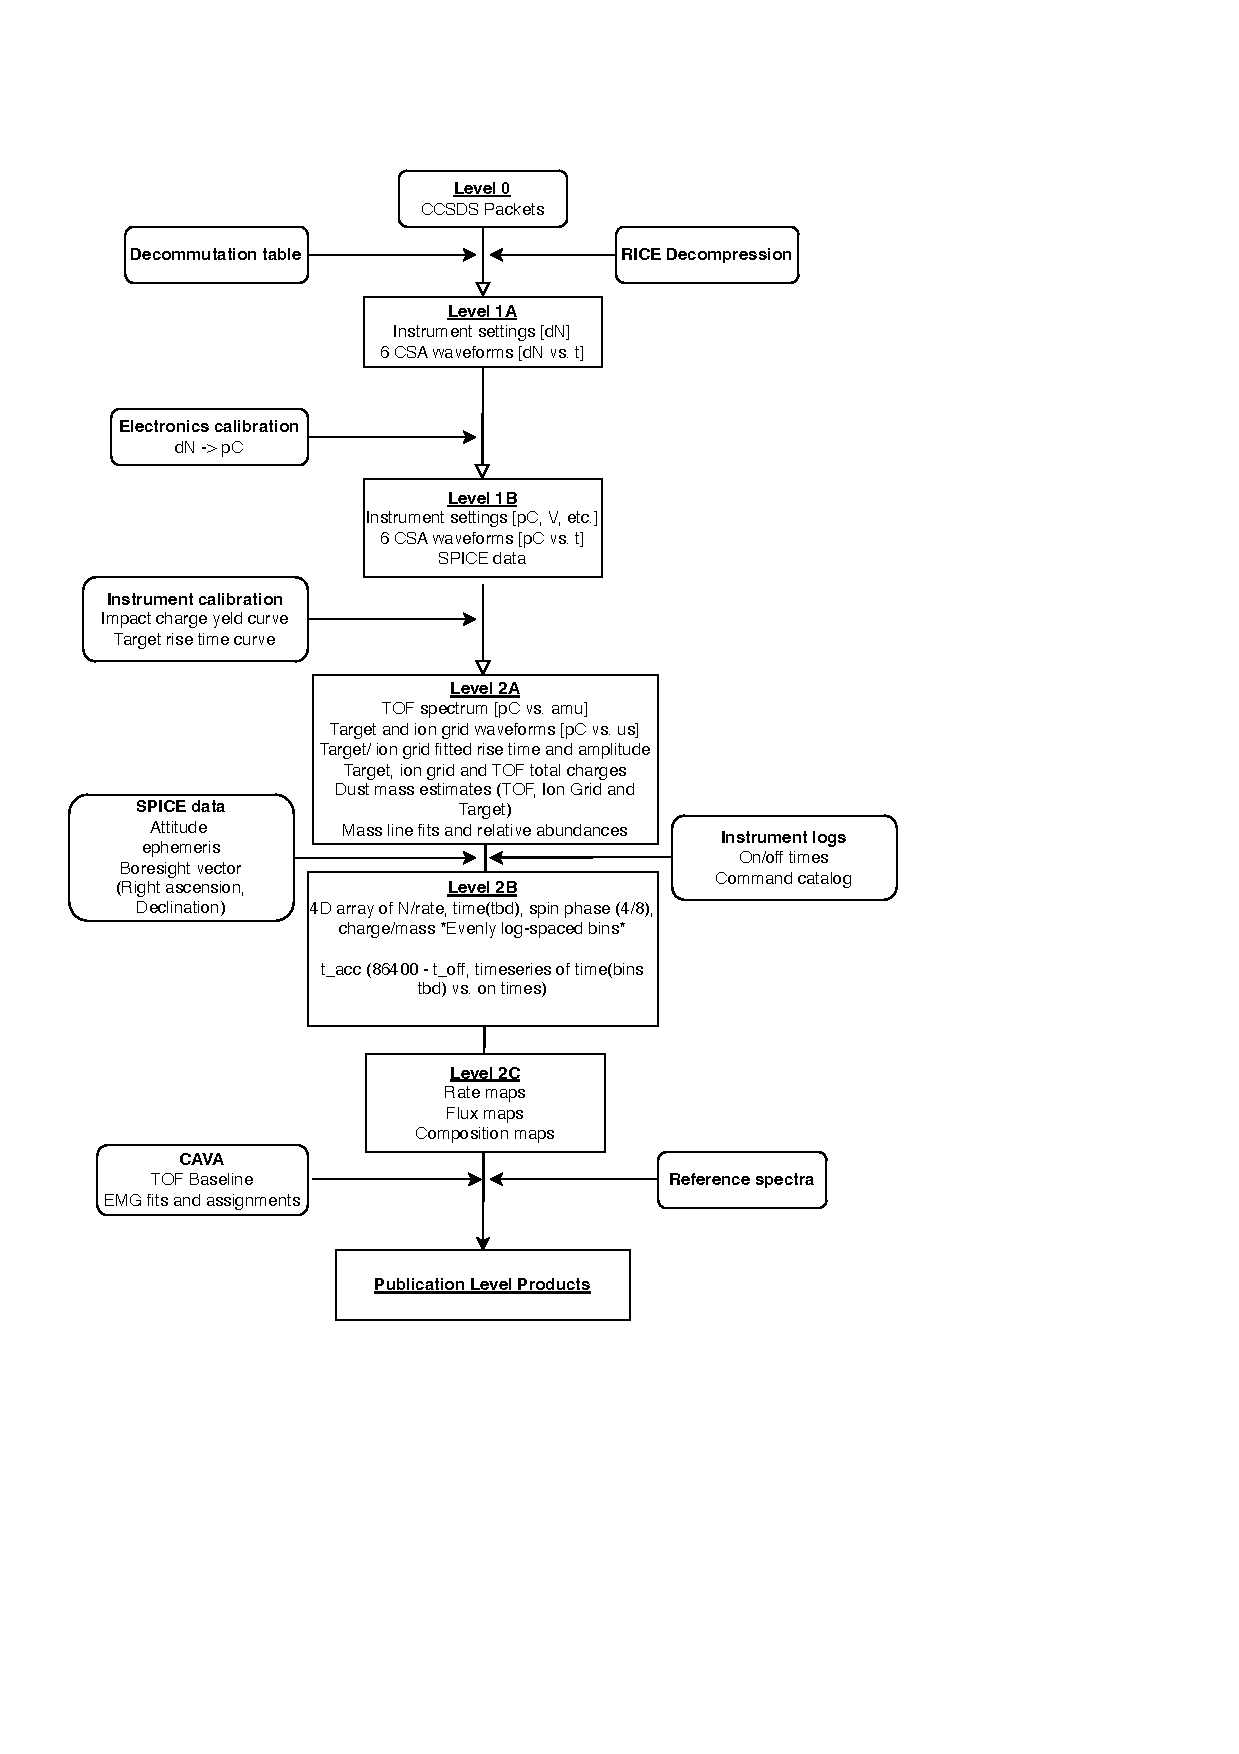
\includegraphics[width=.7\linewidth]{images/PipelineFlow_Updated.key.drawio.pdf}
    \caption{An outline of the IDEX instrument science data product levels, their format, and a brief description.}
    \label{fig:levels}
\end{table}

\subsection{Science Data}
\label{sci}
IDEX generates three APIDs containing science data:
\begin{itemize}
    \item \textbf{Transmit (APID 0x590):} Waveforms and metadata for science events, in response to the \textbf{Transmit} command.
    \item \textbf{Fetch (APID 0x591):} Waveforms and metadata for science events, in response to the \textbf{Fetch} and \textbf{FetchOne} commands.
%    \item \textbf{Catalog (APID 0x592):} Catalog summarizing characteristics of science events for one dataset, in response to the \textbf{SendCatalog} command. (Not implemented for IDEX) %but is available). ????? DO WE DEFINE CATALOG ENTRIES - WHAT IS AVAILABLE?

    
\end{itemize}
The contents of each APID are further described below.  All IDEX packets are 32-bit aligned, starting with a CCSDS header. only APID 0x590 is expected to be used by IDEX.  All IDEX packets are 32-bit aligned, start with a CCSDS header, and end with a 2-byte CRC.  Each IDEX packet is encapsulated in an interface transfer frame (ITF) required by the IMAP General Instrument to Spacecraft Interface Control Document (GI ICD, APL \#7516-9055), but is ignored in this document.
\vspace{.1 in}

In general, science data is organized onboard by the \textbf{accountability identifier (AID)}.  The AID is assigned when the data is acquired, and is used to access the data afterwards.  The AID cannot be changed, and duplicate AIDs are not permitted.  Each dataset is composed of one or more \textbf{“events”}, which is a collection of data collected when the instrument triggers, usually representing a dust particle impact.  Each event is given a unique “event number” by the FPGA, so that every event collected by IDEX can be uniquely identified by the combination of AID and event number. 
\newline





Event data is composed of seven distinct parts:
\begin{enumerate}
\item	Time of Flight (TOF) waveform data on the high-gain (HG) channel, sampled at 260 megasamples per second (Msps) with 10-bit resolution.
\item	TOF waveform data on the mid-gain (MG) channel, sampled at 260 Msps with 10 bit resolution.
\item	TOF waveform data on the low-gain (LG) channel, sampled at 260 Msps with 10 bit resolution.
\item	Ion (ION) grid Charge Sensitive Amplifier (CSA) waveform data, sampled at 4.0625 Msps with 12 bit resolution.
\item	Target Low Range (TLR, AKA target high gain) charge sensitive amplifier (CSA) waveform data, sampled at 4.0625 Msps with 12 bit resolution
\item	Target High Range (THR, AKA target low gain) charge sensitive amplifier (CSA) waveform data, sampled at 4.0625 Msps with 12 bit resolution
\item	FPGA Pre-pended metadata header containing IDEX’s configuration and status at the time of the trigger, recorded by the FPGA.
\end{enumerate}
\begin{figure}[H]
    \centering
    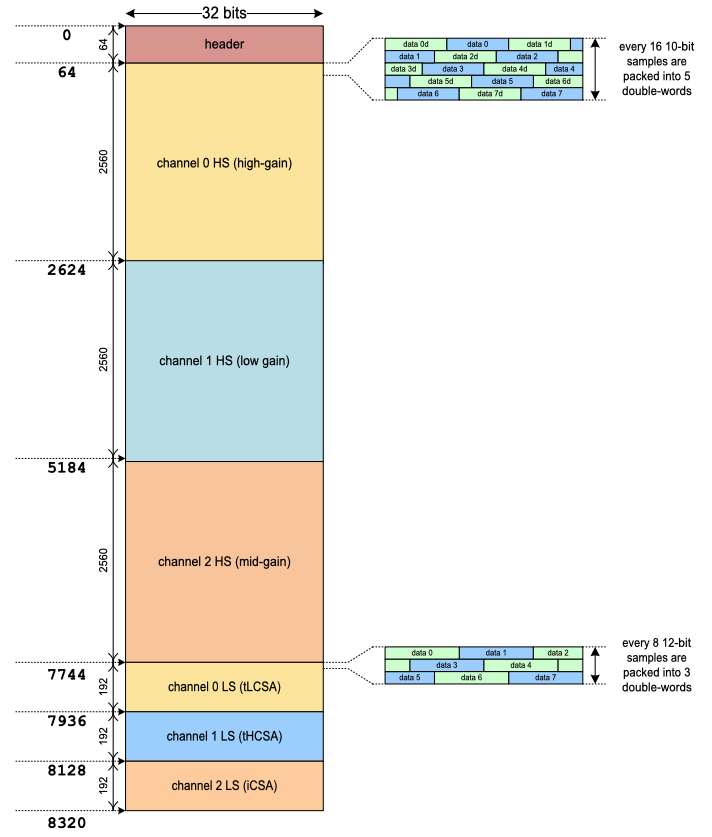
\includegraphics[width=.8\linewidth]{images/waveformdata.png}
    \caption{A bitmap outline of the science data constituting each event}.
    \label{fig:head}
\end{figure}

At the end of science data acquisition, a catalog %WHAT IS IN THE CATALOG?  DO WE DEFINE SPECTRA TYPES ???
representing the new dataset is stored along with the raw science data in nonvolatile memory.  The catalog is mostly empty at this point but can be downlinked with the \textbf{SendCatalog} command.  If no science data is acquired during acquisition, then no catalog is created either. A high-level diagram of how the high and low sampling rate ADC data is transmitted once packetized is shown in Figure \ref{fig:head}, describing how different blocks of data are stored.


Following science data acquisition, FSW will transmit the science data with the “Process\_Transmit” command using APID 0x590. . Processing is started with the \textbf{Process} command, which has the FSW evaluating waveform data to determine characteristics (e.g. peak count) of each event. The characteristics are then used to assign each individual event to a category. As each event in a dataset is processed, a new entry is added to the catalog (in chronological order of acquisition). The FSW includes a setting where event data (all seven parts) are transmitted (APID 0x590) as soon as it is processed – which was used for some early ground testing but never afterward.\newline
A dataset only needs to be processed once but can be processed multiple times (with different results if parameter table entries%DEFINING INSTRUMENT SETTINGS? CHANGED BY WHO WHEN?)
are changed).  However only the most recent processing results are saved to the catalog.\newline
Once a dataset is processed, it can be downlinked as any of the three packet types. Normally the catalog is sent right away since it is considered “feed-forward data” used to configure instrument parameters for subsequent data acquisition opportunities. “Transmitted” science data comes next, and are used as a “first pass” at evaluating the science data and downlinking a subset of acquired events. Afterward, scientists will evaluate the catalog and request specific events to be downlinked as “fetched” science data. Another option is that the dataset can be “transmitted” again but with different parameter table entries resulting in a different selection of events transmitted. %IDEX IS NOT DOING THIS >>>>>PERHAPS ALL CATALOG RELATED STUFF SHOULD BE LEFT OUT?
\newline

\subsubsection{Transmitted and Fetched Science Packets}
Transmitted and fetched science data share the same decommutation, the only real difference being the APID.  When transmitting or fetching science data, one event is handled at a time. Each event may spawn between 1 and 10 packets, depending on size and requested contents. %THIS TOO ONLY MAKES SENSE IF WE HAVE A CATALOG?
\newline
As mentioned above, event data is composed of seven distinct parts but not all are sent for every event.  An argument of the \textbf{FetchOne} command specifies which parts to send, and similarly the Fetch Table includes this info for “Fetch” commands (see \textbf{AddToFetch} command for more details).  Parameter table entries are used to determine what parts of an event are sent for transmitted data (using the event’s category which themselves are grouped into quality factors). % IS THIS  RELEVANT TO IDEX?  MAYBE THERE SHOULD BE A SEPARATE SECTION FOR THE CATALOG STUFF, WHAT IS CATALOGED AND HOW THIS COUD BE USED, AND THAT IT IS NOT EXPECTED TO BE EXERCISED\newline
Each part of the event is packaged into its own packet, while still sharing the same APID.  To fit within the IICD-required maximum CCSDS packet length of 4095 bytes, one packet will contain no more than 4032 bytes of science data (the rest dedicated to headers and such). Each part normally fits in one packet, but the TOF waveforms can span two-three packets if the dataset is large and compression is poor (or disabled). In this case, the maximum amount of science data is sent in the first packet and any leftover sent in the next packet.
The content of packets containing the metadata header are very different from the waveform data, so it is discussed separately.\newline

\subsubsection{Packets Containing Waveforms}
Science packets containing any of the six waveforms, whether transmitted or fetched, start with a brief header and are followed by a variable amount of science data.  The header is never compressed, and provides identifying information such as AID, event number, and which waveform.  \newline
\label{wavepack}
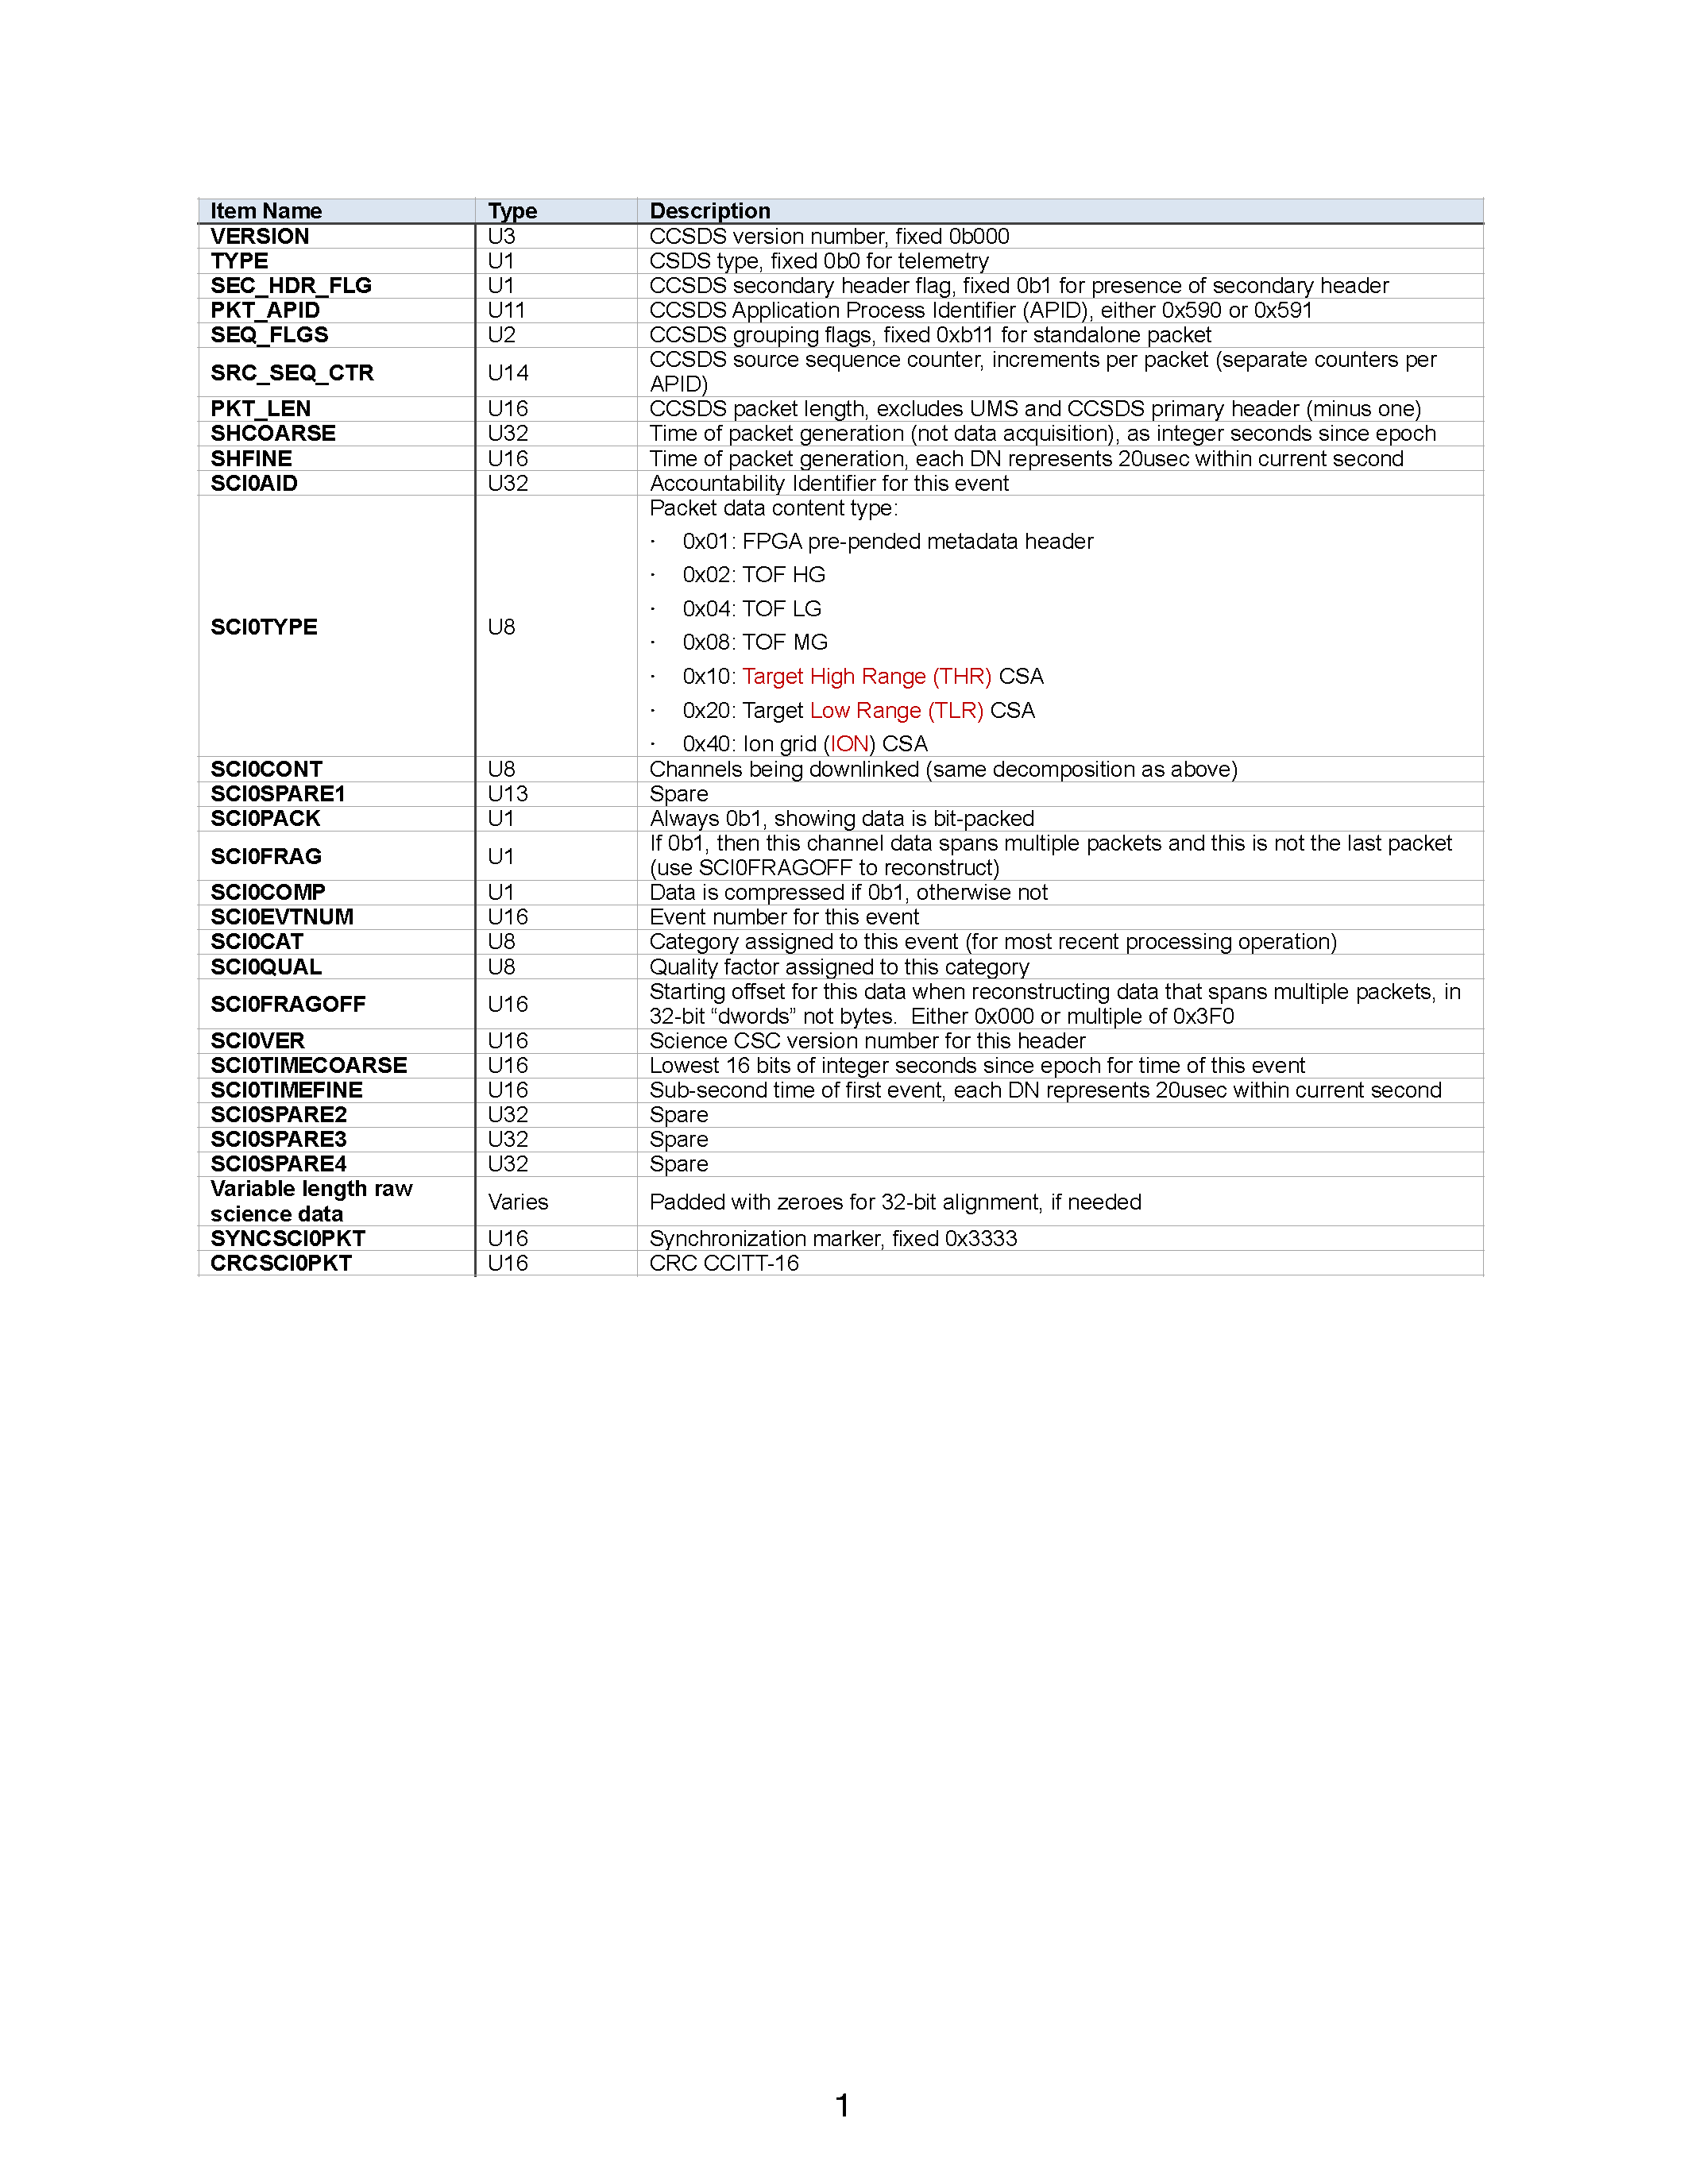
\includepdf[pages=-,pages=1, 
  pagecommand={},
  trim=0 2cm 0 0,
  clip,width=1.25\textwidth]{images/waveformpackets.pdf}

Outline of fields in waveform-containing packets. Red text indicates changes from the SUDA definitions.


\begin{figure}[H]
    \centering
    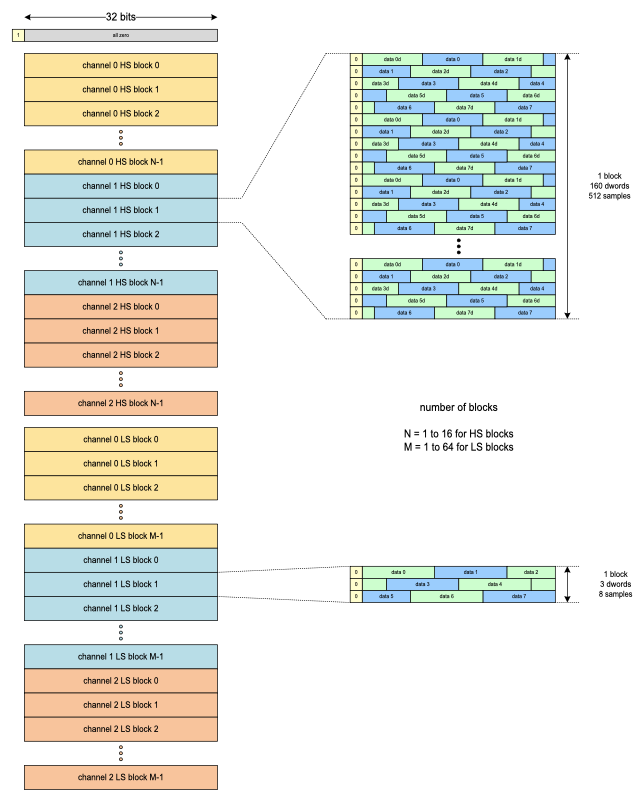
\includegraphics[width=.8\textwidth]{images/wavebreak.png}
    \caption{A bitmap outline of what is contained in each set of waveform data.}
    \label{fig:wavebreak}
\end{figure}

The FSW can make use of the FPGA’s RICE compression core, with details discussed in the FPGA specification (167130). \textbf{If the resulting compressed data is not 32-bit aligned, then the remainder (up to 31 bits) are padded with zeroes}. To decompress a TOF waveform, a RICE decompressor should be used and the output interpreted as a chronological series of 10-bit samples. For SCA %???%
waveforms, the output is 12-bit samples.\newline
After the data is decompressed on the ground, the resulting data represents 6 time-ordered waveforms corresponding to each AID.


The packet is summarized in the table below, using a format similar to the SUDA Command and Telemetry handbook:
\begin{itemize}
    \item Item name: Mnemonic for the named item
    \item Bytes: Position of the item within the element, show bytes with packet and bits within byte
    \item Type of data: Everything is “U” for unsigned data number, followed by bit length
    \item Description: Briefly describes the item, giving the conversion if appropriate.
\end{itemize}
The \textbf{SCI0RAW} field contains the instrument waveforms in each packet. How the header, low sampling and high sampling rate ADC data appears in each packet is described in figure \ref{fig:wavebreak}.
While each channel appears in 3 packets for most events, figure \ref{fig:wavebreak} describes the general case for $N$ high sampling and $M$ low sampling blocks. Each packet header, on the other hand, is only contained in one packet.

\subsubsection{Packets Containing FPGA Metadata Headers}
The packet containing the metadata header holds status and configuration information at the time when this event was acquired. This includes the voltages, currents, temperatures and other instrument settings at trigger time. eThe first 32 bytes after the CCSDS header are identical to the preceding waveform data, so that the SCI0TYPE field can be used as a key to differentiate packets containing this metadata header versus waveforms.

After the common header is the \textbf{FPGA prepended metadata header} that the FPGA captures for every event. These data are fixed size and never compressed.  Many of these fields are the same for all events within the same dataset. A diagram describing the components of the FPGA header is shown in Figure~\ref{fig:headbit}.

\begin{figure}[H]
    \centering
    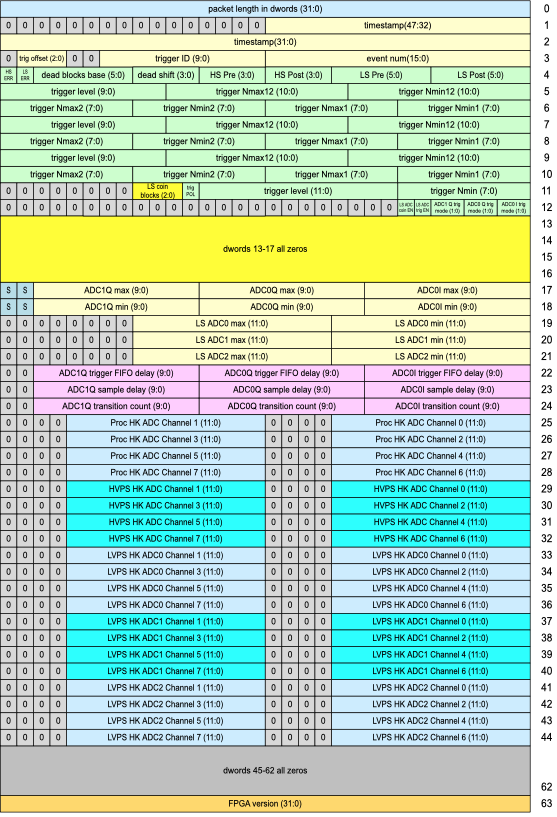
\includegraphics[width=.7\textwidth]{images/HeaderBitmap.png}
    \caption{A bitmap outline of what is contained in each FPGA  metadata event header.}
    \label{fig:headbit}
\end{figure}
The fields in the FPGA header pertinent to the level 0 to 1 science data processing pipeline include the \textbf{timestamp}, \textbf{event num}, and various \textbf{trigger} fields. A full outline of all the available fields including their length, dtype, and description is shown below.

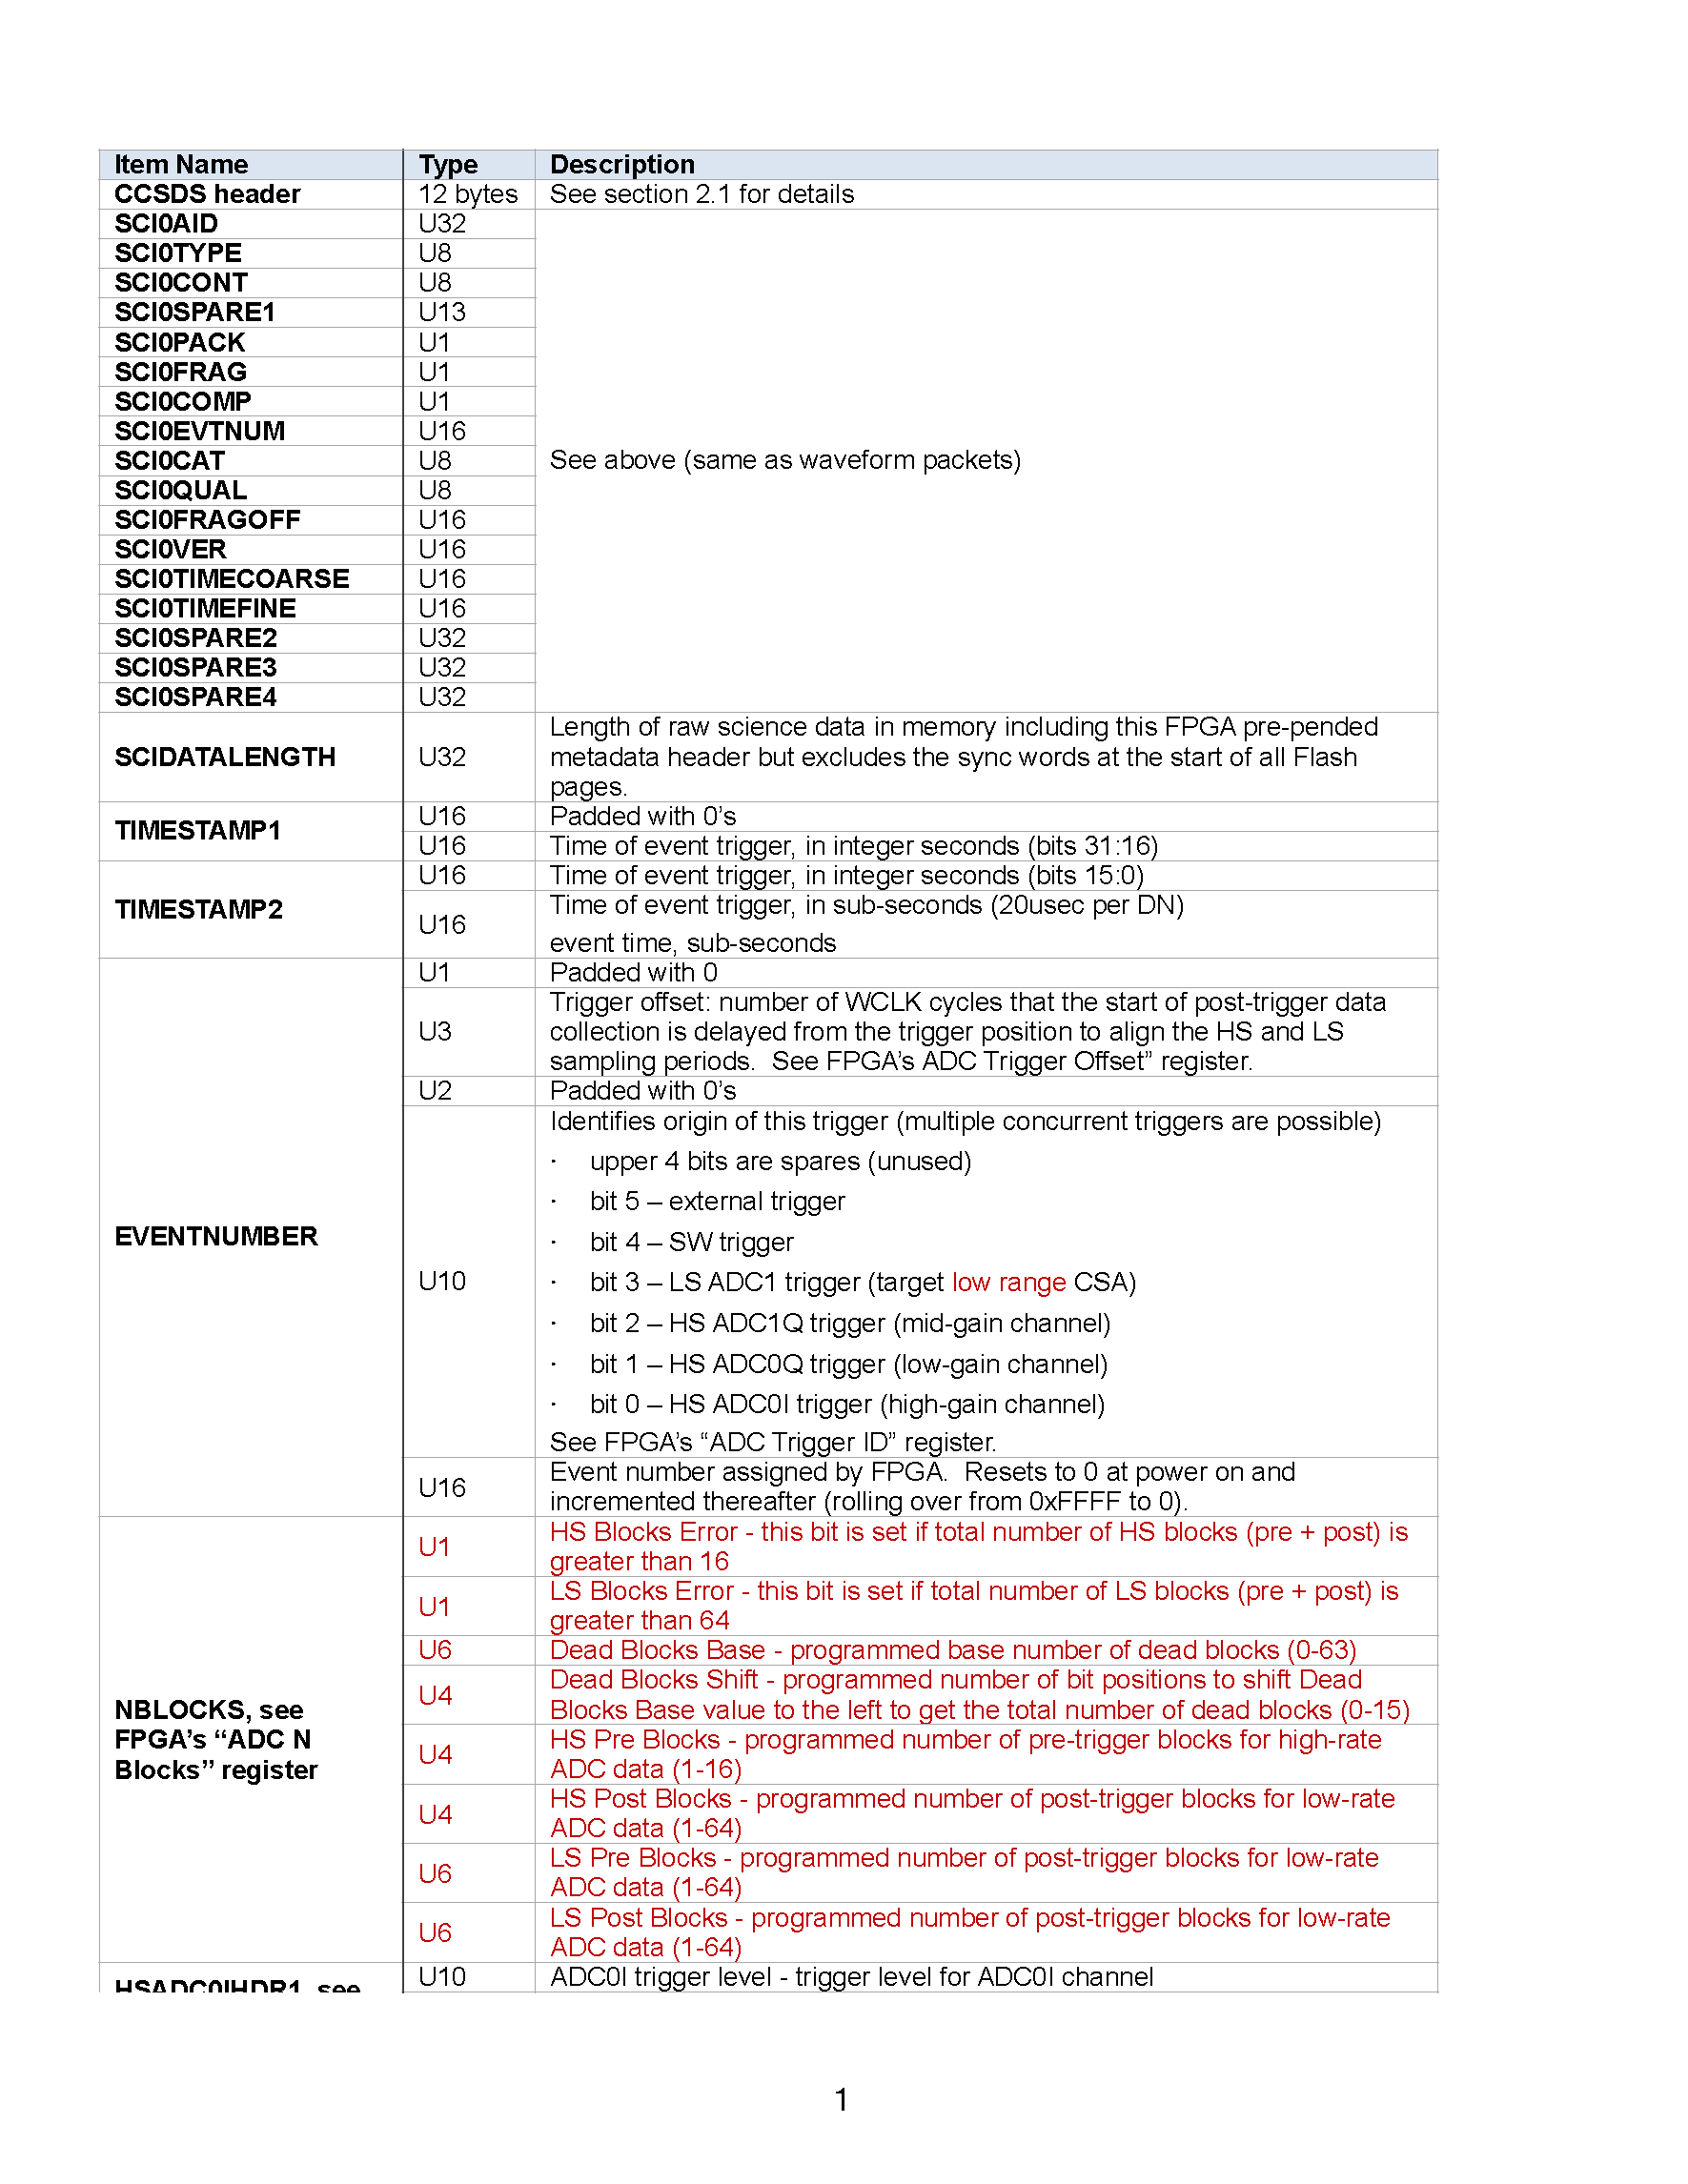
\includepdf[pages=-,width=1.25\textwidth]{images/headerpackets.pdf}


% \subsection{Housekeeping Data}
% ***UPDATE IN FUTURE DRAFT***
% \subsection{Engineering Mode Data}
% ***UPDATE IN FUTURE DRAFT***
% \subsection{In-Flight Calibration Data}
% ***UPDATE IN FUTURE DRAFT***


\chapter{Data Processing} 
\label{chap:chap5}
This chapter describes the necessary steps to convert data between each of the levels described in the processing flowchart. Source code snippets are provided in Python.
\section{Overview}
The IDEX data processing pipeline takes the data packets described above, an xml XTCE definition/decommutation table (\ref{xtce}), the instrument ground calibration curve, the spacecraft thruster data, and ephemerides data as inputs. Each data product and its corresponding inputs/outputs is described in Figure \ref{fig:flow}.

\begin{figure}[H]
    \centering
                                                                                                                                                                                                                             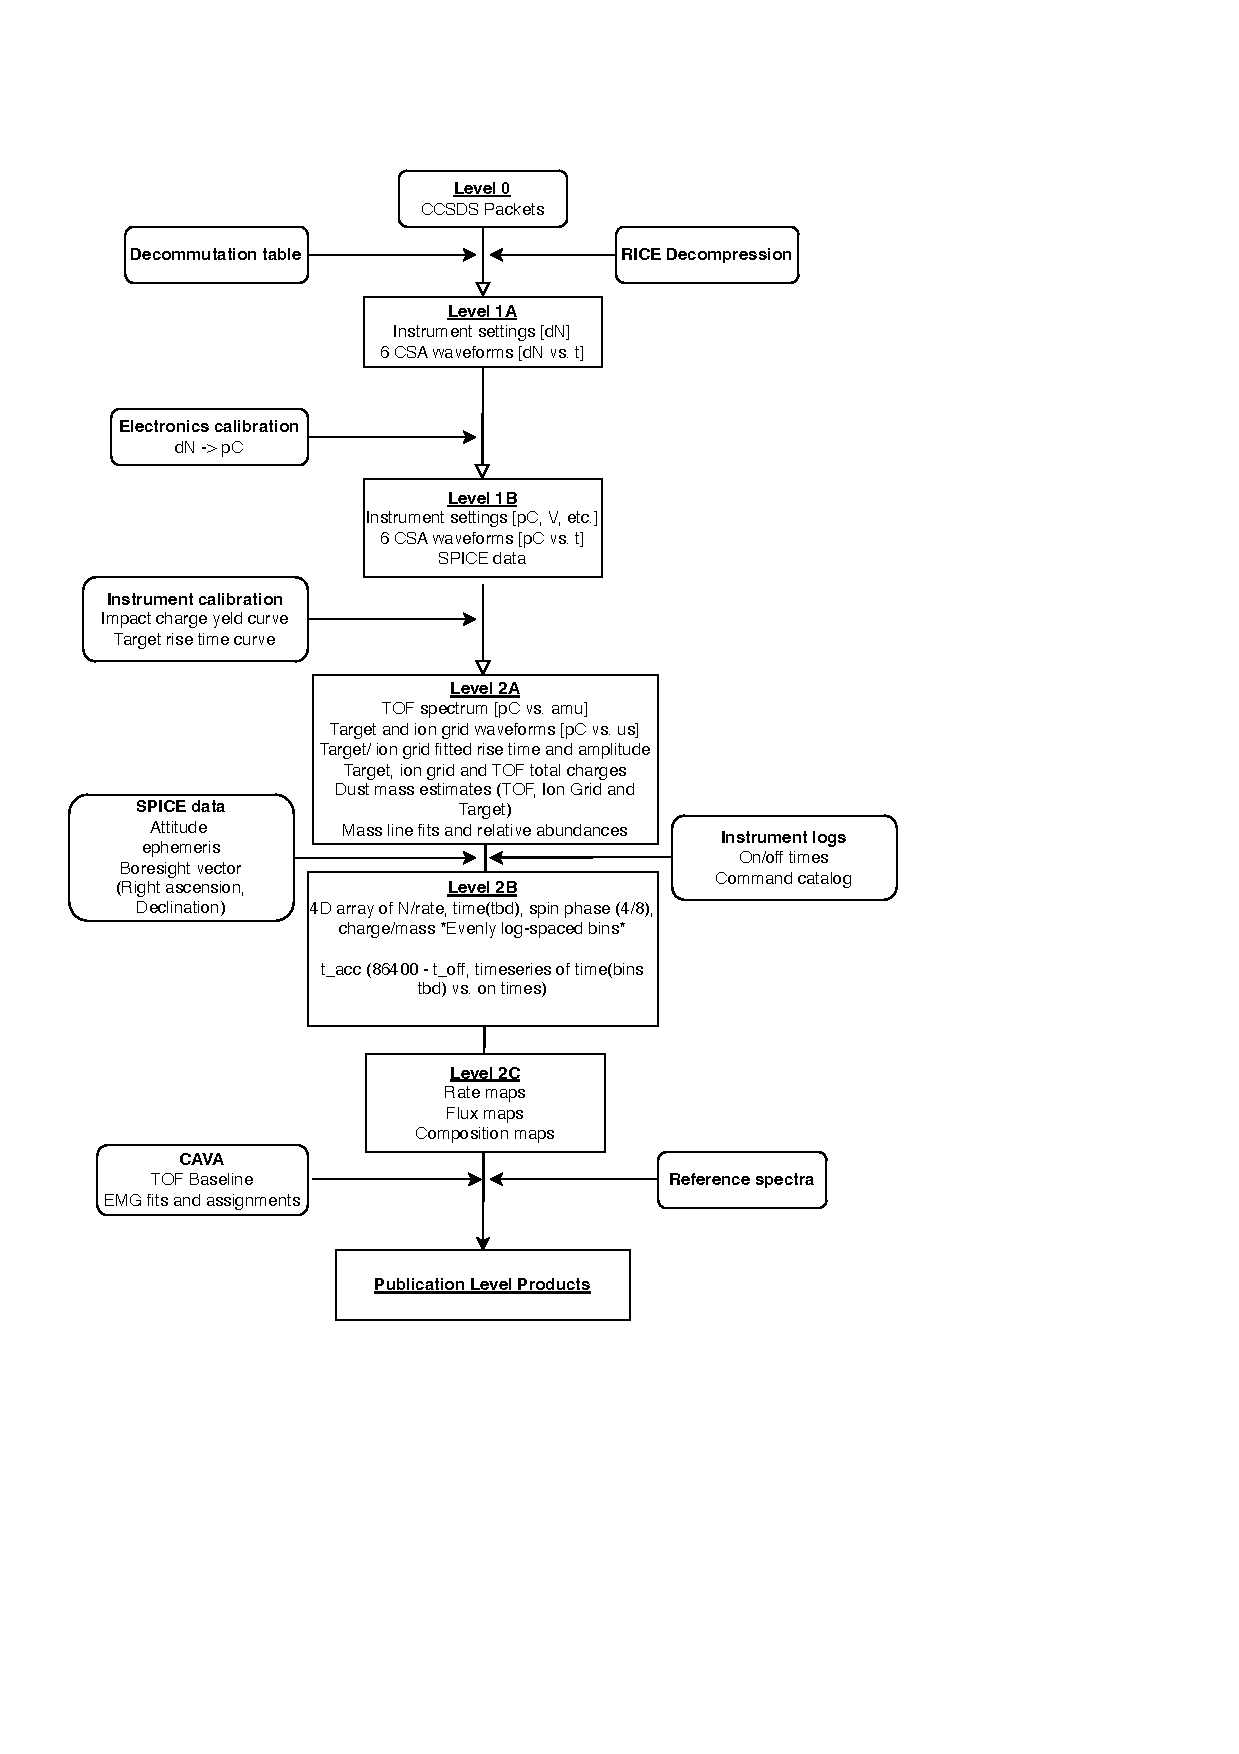
\includegraphics[width=.7\linewidth]{images/PipelineFlow_Updated.key.drawio.pdf}
    \caption{The IDEX science data pipeline processing flowchart. Data products are given in the center, with the necessary auxiliary inputs on the sides.}
    \label{fig:flow}
\end{figure}

\section{Data Volume Expectancy}

The estimates for the expected IDEX instrument science data volume are derived from simulations of known IDP and ISD populations. Figure \ref{fig:isdpop} depicts counts for ISD (red/blue) and IDP (black) particles expected to be measured by IDEX during the mission.

\begin{figure}[H]
    \centering
    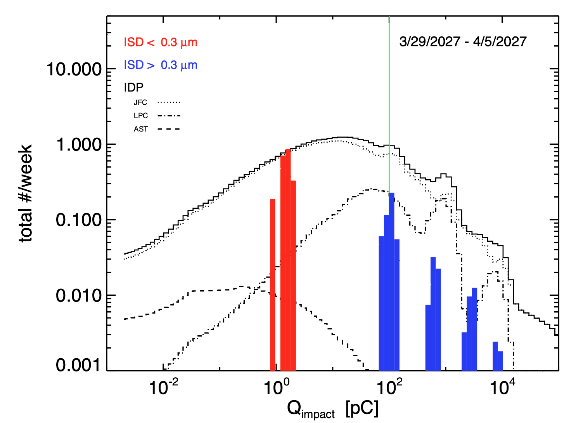
\includegraphics[width=.7\linewidth]{images/IDPISD.png}
    \caption{Expectations for IDEX's ISD and IDP measurements during the mission. Note that although this is just shown for 6 days in 2027, these simulations have been carried out for all of the prime and extended IMAP mission.}
    \label{fig:isdpop}
\end{figure}

From this simulation, IDEX is expected to measure 16 events per day on average. Using these estimates in conjunction with the bitmap in Figure \ref{fig:headbit}, we can estimate the weekly data volume expectancy for IDEX during the mission. This has been carried out for each of the science data product levels, as depicted in table \ref{fig:vol}.

\begin{table}[H]
    \centering
    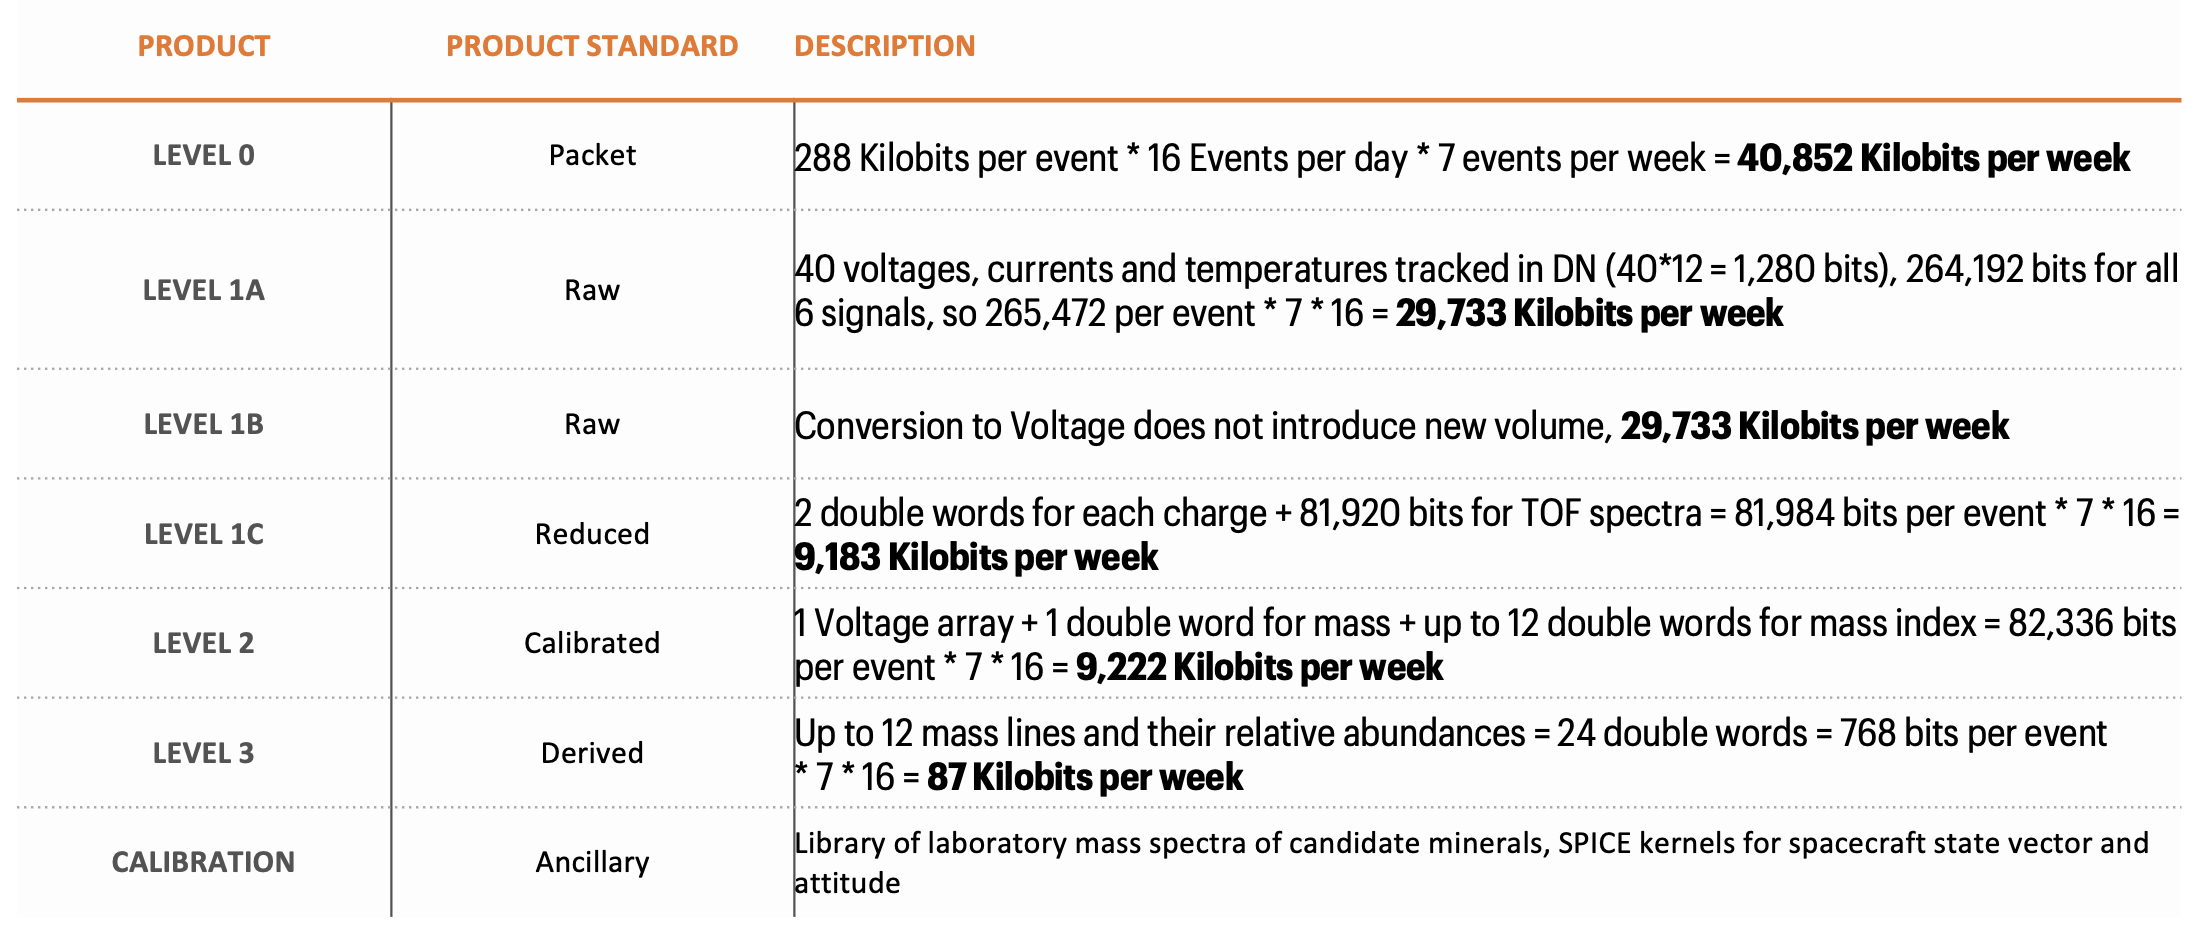
\includegraphics[width=\linewidth]{images/DataVolume.png}
    \caption{Expectations for IDEX's weekly data volume throughout the mission, organized by data product level.}
    \label{fig:vol}
\end{table}


\section{Heritage Data Processing}
IDEX has a high-level of heritage from the SUrface Dust Analyzer (SUDA) onboard the upcoming flagship \textit{Europa Clipper} mission. SUDA is nearly identical but has instead been optimized for flybys and detections of organic molecules for a limited impact velocity range of around 4 km/s.  The XTCE definition is the same for both instruments (see appendix \ref{xtce}), but the interpretation of the waveforms differs, along with voltage/temperature conversions.

Like IDEX, SUDA Event data is composed of seven distinct parts:
\begin{enumerate}
\item	Time of Flight (TOF) waveform data on the high-gain (HG) channel, sampled at 250 megasamples per second (Msps) with 10 bit resolution
\item	TOF waveform data on the mid-gain (MG) channel, sampled at 250 Msps with 10 bit resolution
\item	TOF waveform data on the low-gain (LG) channel, sampled at 250 Msps with 10 bit resolution
\item	Velocity (Qv) grid charge sensitive amplifier (CSA) waveform data, sampled at 3.75 Msps with 12 bit resolution
\item	Ion (Qi) grid CSA waveform data, sampled at 3.75 Msps with 12 bit resolution
\item	Target (Qt) CSA waveform data, sampled at 3.75 Msps with 12 bit resolution
\item	FPGA Pre-pended metadata header containing IDEX’s configuration and status at the time of the trigger, recorded by the FPGA
\end{enumerate}

The velocity grid CSA takes the place of IDEX's second target gain stage. Otherwise, the names, sampling rates, and bit resolutions are all identical. SUDA leverages the use of the SWIFT language-based SPECTRUM software, developed in-house at LASP. To avoid this Mac OS dependency, the IDEX pipeline has been constructed exclusively in Python 3.8.
\section{Level 0 to Level 1A Processing}
\subsection{Decommutation}
Packet decommutation relies on the \textbf{LASP packets} library, available on the \href{https://bitbucket.lasp.colorado.edu/projects/SDS/repos/lasp_packets/browse}{LASP Bitbucket (LASP VPN access required)}. The \textbf{LASP packets} software hinges on the \textbf{generator} method of the \textbf{Parsing.PacketParser} module for reading CCSDS packets (please see appendix \ref{lasppackets} for Python source code).

The packet data is read in using Python's \textbf{bitstring} library to reduce memory usage. Each packet is associated with a "flattened sequence container" from the XTCE definition. To do this, first, the length of the packet is taken from the CCSDS header:

\begin{minted}[breaklines, xleftmargin=20pt]{python}
specified_packet_data_length = self._total_packet_bits_from_pkt_len(header['PKT_LEN'].raw_value)
\end{minted}

Next, the type of packet as provided by the CCSDS header is cross-referenced with the XTCE definition to find a matching APID, VERSION, and TYPE. If there is a match, the code parses the packet according to the XTCE definition. If there is no match, it will attempt to generally parse it using the length of the packet. The source for this is shown below.

\begin{minted}[breaklines, xleftmargin=20pt]{python}
try:
                if isinstance(self.packet_definition, xtcedef.XtcePacketDefinition):
                    packet = self.parse_packet(binary_data,
                                               self.packet_definition.named_containers,
                                               root_container_name=root_container_name,
                                               word_size=self.word_size)
                else:
                    packet_def_name, parameter_list = self._determine_packet_by_restrictions(header)
                    packet = self.legacy_parse_packet(binary_data, parameter_list, word_size=self.word_size)

\end{minted}

This process is repeated until we have parsed each of the packets in the dataset.

\subsection{Science Data}
Once the data has been depacketized, the \textbf{SCI0TYPE} field designates what data is contained in each packet. Per the table in \ref{wavepack}, the possible values of \textbf{SCI0TYPE} include:
\begin{mdframed}[backgroundcolor=backcolour]{
 {\bf 1} = FPGA pre-pended metadata header \\
 {\bf 2} = TOF HG \\
 {\bf 4} = TOF LG \\
 {\bf 8} = TOF MG \\
 {\bf 10} = Target LG ($Q_T$) CSA \\
 {\bf 20} = Target HG ($Q_T$) CSA \\
 {\bf 40} = Ion grid ($Q_I$) CSA \\
} \end{mdframed}

By reading in the \textbf{SCI0TYPE} field, the appropriate ADC sampling rate (and therefore bit pattern) is determined.
\newpage 
The waveform data must be read in a pattern specific to high or low sampling rate ADCs in the schema outline below:

\begin{mdframed}[backgroundcolor=backcolour]{
\large For \textbf{high sampling rate (TOF) data (10-bit samples)}, handle the raw data as 32-bit units like this (most significant bit first):\newline 
\normalsize \\
  {\bf 2 bits} = Padding set to zeros, ignore this \\
  {\bf 10 bits} = oldest sample \\
  {\bf 10 bits} = next sample \\
  {\bf 10 bits} = next (newest) sample \\ 
\newline
\noindent \large For the remaining \textbf{low sampling rate data (12-bit samples)}, handle the raw data as 32-bit units like this (most significant bit first):\newline 
 \normalsize \\
  {\bf 8 bits} = Padding set to zeros, ignore this \\
  {\bf 12 bits} = oldest sample \\
  {\bf 12 bits} = next (newest) sample \\
} \end{mdframed}

Once this schema has been used for the waveform data, all the science event data has been read in and stored. The example Python script below will read in an IDEX raw binary data file, plot each of the event waveforms, and write all of the data to an easily accessible HDF5 file. Plots are saved to a \textit{/Plots/} directory in the same directory as the script, and the HDF5 files are written to the \textit{/HDF5/} directory.


It has been updated to be used as a command line tool, so we may use:
\begin{minted}[breaklines]{python}
python idex_packet.py --file filename
\end{minted}
Where $filename$ must be replaced with the name of the packet file, and $python$ must be an alias for a python installation. The $--file$ can be substituted for $-f$.

\subsection{Metadata translation and timing validation}
The HDF5 writer now mirrors the FPGA header layout in two dedicated subgroups beneath \textit{/Metadata/}: \textit{/Metadata/raw/} contains the raw field names and integer payloads exactly as they appear in the FPGA table (\texttt{IDX\_\_SCI0TIME32}, \texttt{IDX\_\_TXHDRSAMPDELAY}, \texttt{IDX\_\_TXHDRTRIGOFFSET}, etc.), while \textit{/Metadata/unpacked/} carries the decoded quantities used throughout the analysis (timestamp seconds/subseconds, trigger level/mode, per-channel sample delays, and pre-trigger block counts). The unpacked entries are also aliased to the legacy paths directly under \textit{/Metadata/} so existing notebooks continue to resolve fields like \textit{Epoch} or \textit{TriggerLevel}. The raw-to-unpacked pairing lets reviewers validate the algorithms template against flight data by comparing each raw integer to its derived counterpart in a single event.

Time handling is now fully derived from the FPGA header. The 32-bit \texttt{IDX\_\_SCI0TIME32} coarse counter advances in 20~$\mu$s increments; \texttt{TimestampSeconds} and \texttt{TimestampSubseconds} are derived by separating the integer seconds from the remaining fractional portion (scaled by 50{,}000 counts/s), and an \texttt{Epoch} value in milliseconds is retained for convenience. The helper routine preserves monotonicity across counter rollovers by tracking the 2$^{32}$\,$\times$\,20~$\mu$s period, and it honours an optional file-based anchor time to keep sequences within the intended day. Trigger alignment uses three additive pieces: (1) a pre-trigger window based on the HS/LS block counts from \texttt{IDX\_\_TXHDRBLOCKS}, (2) the WCLK-based trigger offset in \texttt{IDX\_\_TXHDRTRIGOFFSET} (scaled by $1/32.5$ to yield a $\approx$30.8~ns increment), and (3) the per-channel sample delays from \texttt{IDX\_\_TXHDRSAMPDELAY} and the FIFO delay (\texttt{IDX\_\_TXHDRFIFODELAY}) expressed in $1/260$~$\mu$s units. These terms are injected directly into the \textit{Time (high sampling)} and \textit{Time (low sampling)} datasets, so the $t=0$ crossing in each waveform now reflects the firmware’s reported offsets.

\begin{table}[H]
\centering
\renewcommand{\arraystretch}{1.15}
\begin{tabular}{|p{3.4cm}|p{3.8cm}|p{4.8cm}|p{4.2cm}|}
 \hline
 \rowcolor{darkGrey}\textcolor{white}{\textbf{FPGA field}} & \textcolor{white}{\textbf{HDF5 raw path}} & \textcolor{white}{\textbf{Unpacked path \& quantity}} & \textcolor{white}{\textbf{Translation / timing note}} \\\hline
 \texttt{IDX\_\_SCI0TIME32} & \textit{/Metadata/raw/IDX\_\_SCI0TIME32} & \textit{/Metadata/unpacked/\{SCI0Time32, TimestampSeconds, TimestampSubseconds, Epoch, SpacecraftSeconds\}} & 32-bit counter in 20~$\mu$s units; rollovers corrected before splitting integer seconds from fractional subseconds (50{,}000 ticks/s). Epoch retains the millisecond value used by downstream plots. \\\hline
 \texttt{IDX\_\_SCI0TYPE}, \texttt{IDX\_\_SCI0AID}, \texttt{IDX\_\_SCI0EVTNUM} & \textit{/Metadata/raw/(field name)} & \textit{/Metadata/unpacked/\{SCI0Type, SCI0AID, SCI0EventNumber\}} & Packet routing metadata used to classify each waveform and preserve the AID alongside the event counter. \\\hline
 \texttt{IDX\_\_TXHDRBLOCKS} & \textit{/Metadata/raw/IDX\_\_TXHDRBLOCKS} & \textit{/Metadata/unpacked/\{HSPretriggerBlocks, HSPosttriggerBlocks, LSPretriggerBlocks, LSPosttriggerBlocks, HSPretriggerOffsetMicroseconds, LSPretriggerOffsetMicroseconds\}} & Block counts define the pre-trigger window: HS offsets subtract $512/260$~$\mu$s per block, LS offsets subtract $8/4.0625$~$\mu$s per block before zeroing the time axis. \\\hline
 \texttt{IDX\_\_TXHDRTRIGOFFSET} & \textit{/Metadata/raw/IDX\_\_TXHDRTRIGOFFSET} & \textit{/Metadata/unpacked/\{TriggerOffsetTicks, TriggerOffsetMicroseconds\}} & WCLK cycles (32.5~MHz) reported by firmware; converted to $\mu$s and added to every time base to preserve the firmware-defined trigger instant. \\\hline
 \texttt{IDX\_\_TXHDRSAMPDELAY} & \textit{/Metadata/raw/IDX\_\_TXHDRSAMPDELAY} & \textit{/Metadata/unpacked/SampleDelayMicroseconds\_TOF\_\{H,M,L\}} & Three 10-bit fields encode channel-specific sample delays at the 260~Msps rate (3.85~ns per tick). Each delay shifts its corresponding TOF channel before fitting or mass-line extraction. \\\hline
 \texttt{IDX\_\_TXHDRFIFODELAY} & \textit{/Metadata/raw/IDX\_\_TXHDRFIFODELAY} & \textit{/Metadata/unpacked/FIFODelayMicroseconds} & FIFO latency applied to low-rate channels, scaled by $1/260$~$\mu$s to keep the ion grid and target CSAs aligned with the TOF streams. \\\hline
 \texttt{IDX\_\_SCI0RAW} waveform words & Captured via \textit{/Data/} then written to channel datasets (\textit{/event/TOF H}, \textit{/event/Target L}, etc.) & \textit{/Time (high sampling)}, \textit{/Time (low sampling)} arrays share the same offsets and delays as the channel data & Rice-decompressed into 10-bit (TOF) or 12-bit (CSA) sample arrays, with the above timing corrections baked into the saved time axes for each channel. \\\hline
\end{tabular}
\caption{Mapping between FPGA header fields, their raw HDF5 storage, and the derived “unpacked” quantities used by the processing software.}
\label{tab:fpga_to_packet}
\end{table}


\subsection{Housekeeping data}
The IDEX instrument settings delineated in table **** are all decommutated and stored with their raw DN values in the CDF file for level 1A.
% ***UPDATE IN FUTURE DRAFT***

\section{Level 1A to Level 1B Processing}
Level 1B data contains both instrument settings and waveforms in physical units, rather than in dN. For the waveforms, a linear transformation is used to convert to pC. These values have been established for the IDEX FM, and are tabulated in~\ref{table:dntopc}.


\begin{table}[h!]
\caption{IDEX Flight Gains, updated on 10/10/24.\\}
\centering
\begin{tabular}{c|c|c|c|c}
 \hline \hline
  & Variable  & Conv. Factor & Sampling Rate  & Bits \\ 
  & (pC/DN)  & (pC/DN) & (MHz)  &  \\ \hline\hline
 \textbf{High Gain TOF}   &  $Q_{tof,tot}$   & $2.89 \times 10^{-4}$ &  260  &  10 \\ \hline
 \textbf{Mid Gain TOF}   &  $Q_{tof,tot}$  & $1.13 \times 10^{-2}$ &  260  &  10 \\ \hline
 \textbf{Low Gain TOF}   &  $Q_{tof,tot}$  & $5.14 \times 10^{-1}$ &  260  &  10 \\ \hline
 \textbf{Ion Grid}   &   $Q_{iG}$   &   $7.46 \times 10^{-4}$ & 4.0625 &  12 \\ \hline
 \textbf{Target High Gain}   &  $Q_{tgt}$   &  $1.63 \times 10^{-1}$ & 4.0625 &  12 \\ \hline
 \textbf{Target Low Gain}   &  $Q_{tgt}$   &    $1.58 \times 10^{1}$ & 4.0625 &  12 \\ \hline
\end{tabular}
\label{table:dntopc}
\end{table}

A polynomial transformation is used to convert the instrument settings from dN to physical units. Below is a table of all the instrument settings and their polynomial conversion values.

% \includepdf[pages=-]{images/IDEX_CDF_Variable_Definitions.pdf}

Here, (C0,C1,...) are the coefficients for the polynomial transformation. The equation to transform from dN to physical units is then

\begin{equation}
    P(dN) = \sum_{0}^{i} C_{i}(dN)^{i},
\end{equation}
where $P$ is the value in physical units and $dN$ represents the value in dN.


\section{Level 1B to Level 2A Processing}
The transition from 1B to 2A involves performing fits to each of IDEX's signals, then deriving quantities from those fit parameters to estimate the mass, speed and composition of the impacting dust particle.

\subsubsection{Target and Ion Grid Signal Fits}
The level 1B to 2A conversion uses fits to the ion grid and two target signals to estimate the total impact charge generated by the dust particle. The mass and speed are derived from these fit parameters and our calibration data.

The fit function is given by (Horányi, 2014), \begin{equation}
    y(t; t_{0}, C_{0}, C_{1} , C_{2}, \tau_{0}, \tau_{1}, \tau_{2}) = C_{0} + H(t-t_{0})[C_{2} \big(1-e^{-\frac{t-t_{0}}{\tau_{1}}} \big) e^{-\frac{t-t_{0}}{\tau_{2}}} - C_{1}]
\end{equation}

where $H(t-t_{0})$ is the Heaviside function. Here, $C_{0}$ s the initial baseline.

The impact charge is calculated by taking the difference between the initial baseline and the peak of the signal. An example fit for the ion grid signal is depicted in figure \ref{fig:targetfit}.

% This plot should be in the IDEX cadence/sampling rate, and should have lines indicating what I mean by the peak and the baseline.
\begin{figure}[H]
    \centering
    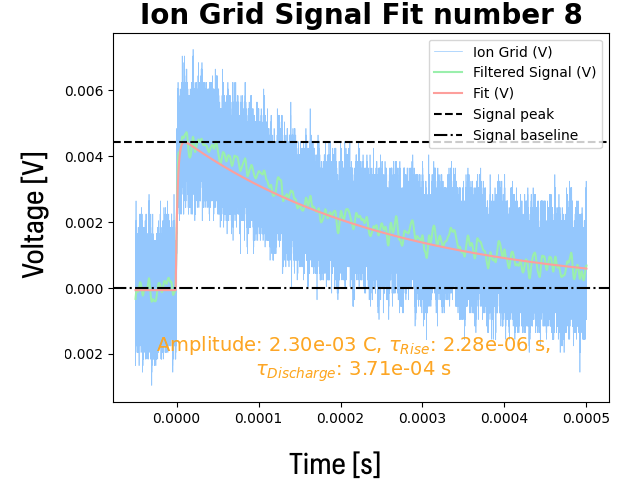
\includegraphics[width=6.5 in]{images/TargetSignal.png}
    \caption{An example fit to the target signal. The original signal is blue, the filtered signal is given in green and the fit is the red curve. The fit parameters are displayed in orange text.}
    \label{fig:targetfit}
\end{figure}

Prior to performing the target signal fit, the two gain stages (target low gain, target high gain) have to be combined into one signal. This is done by subtracting an average of the first 10 points from both signals to correct for the offsets in [dN]. Then, the low- and high-gain target signals are scaled by their respective pC/dN conversion values, given in \autoref{table:dntopc}. An example result where the target high gain channel saturates and is shown in \autoref{fig:combinedtarget}.

\begin{figure}[H]
    \centering
    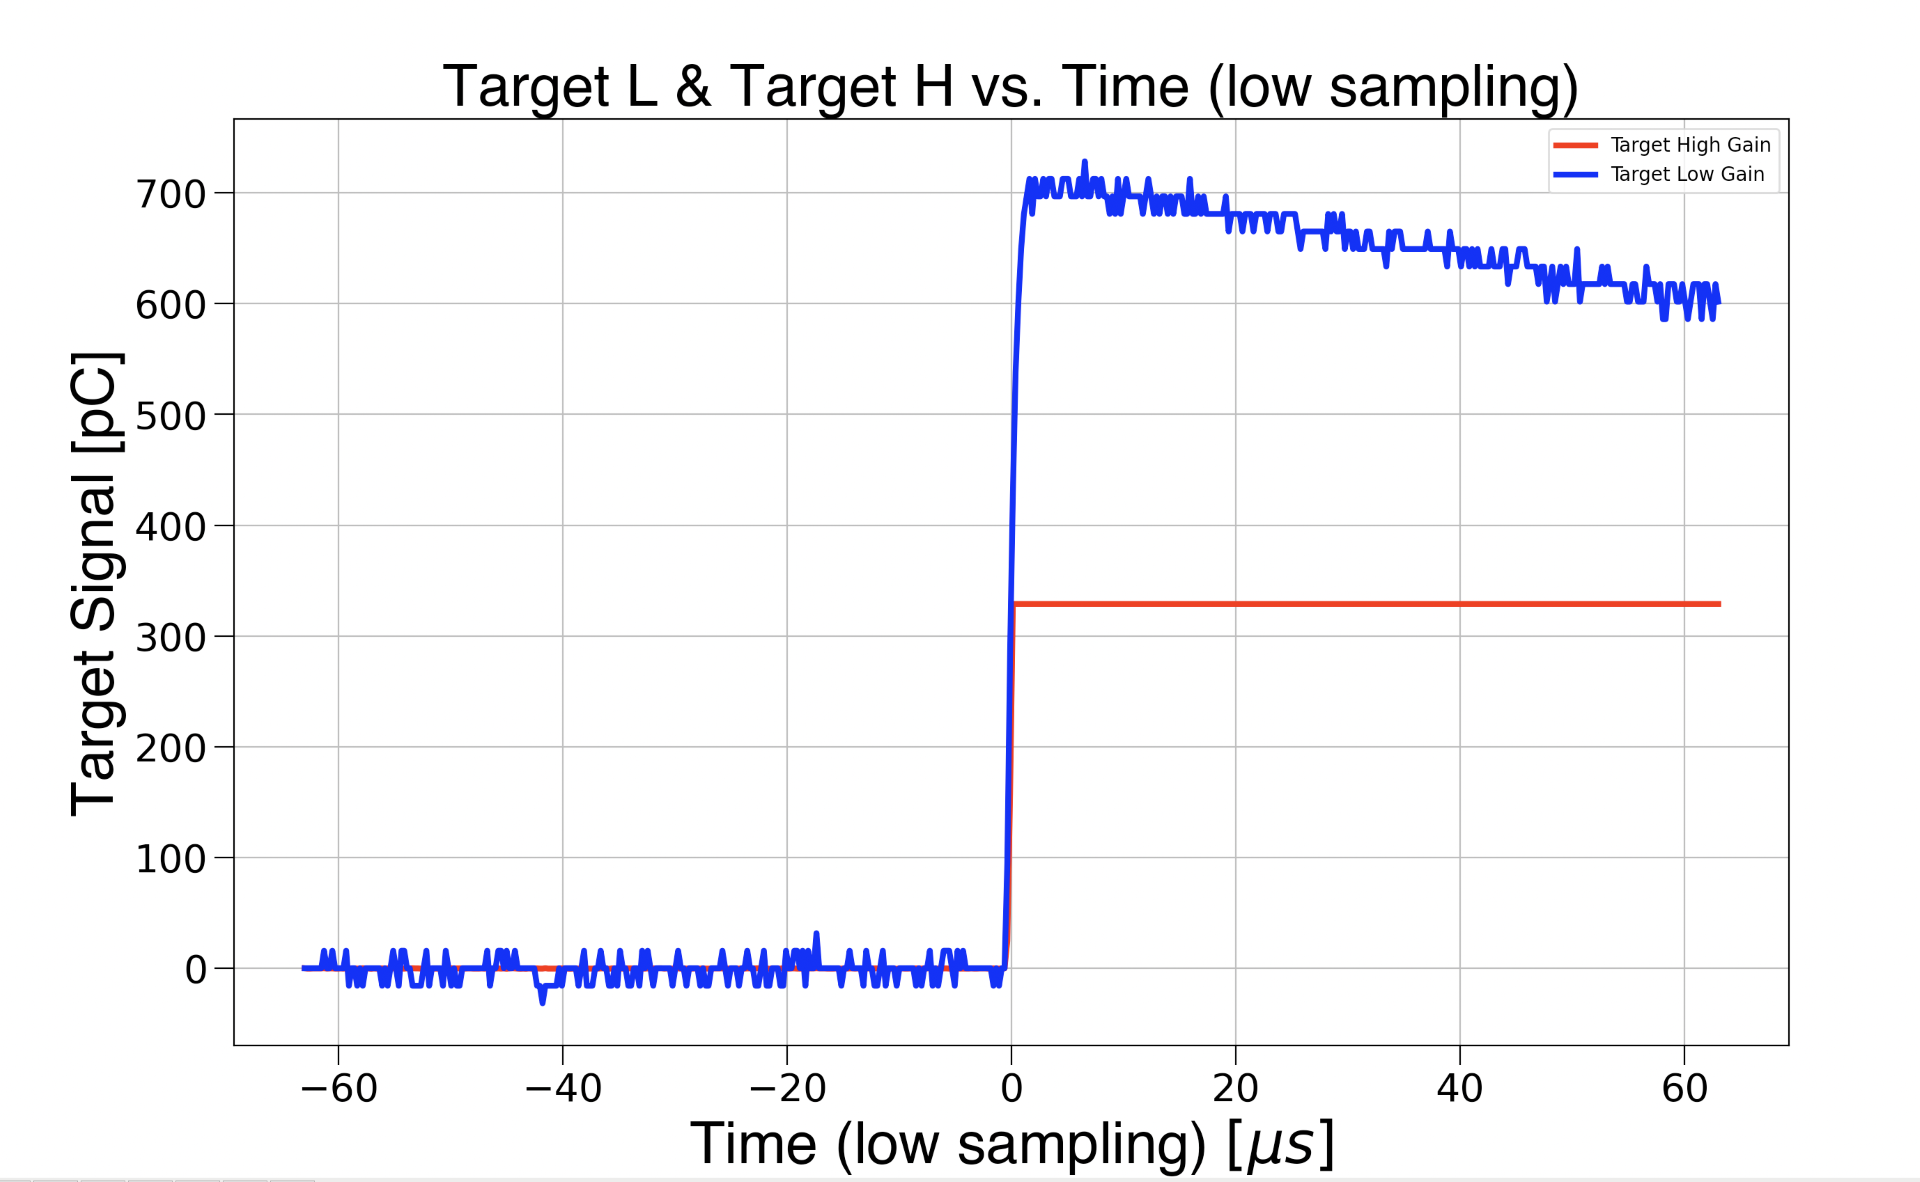
\includegraphics[width=6.5 in]{images/combined_target_signals.png}
    \caption{An example of combined target signals from Aluminum (Al) dust testing on the IDEX FM with the FM CSAs.}
    \label{fig:combinedtarget}
\end{figure}
Here, the target low gain (blue) is considered, as the high gain (red) saturates at 328.8 pC. The pC values \textbf{(in the specific case of the flight model with the flight CSAs)} were obtained from \autoref{table:dntopc} and are .163 and 15.8357 [pC/dN] for the high and low gain channels, respectively. 

Designate the best waveform (single or combined) with a flag for how it was created ("fit data"). Put this in a flag that can represent any permutation.

The dust mass can be estimated from the numerical integral of the combined TOF spectrum and signal fits to combined target and ion grid channels. The dust particle's impact charge is proportional to both its mass and velocity (Collette, 2014). It is estimated by the amplitude of both the target and ion grid signals, and by the integral of the TOF spectrum. The total charge (\(Q_i\)) generated during a dust impact of mass \(m\), at velocity \(v\)) follows the power law
\begin{equation}
Q_{i} \propto m^{\alpha} v^{\beta},
\end{equation}
where the exponents \(\alpha\) and \(\beta\) vary with the composition of the target and projectile and are experimentally derived. Typical values for $\alpha$
 and $\beta$ fall between 1-2 and 2-5, respectively. 

 \begin{equation}
Y(v; A, a_1, a_2, a_3, v_b, v_c, k) = A\cdot v^{a_1}\left [ \left(1+(\frac{v}{v_b})^k\right)^{\frac{a_2 - a_1}{k}} \cdot \left(1+(\frac{v}{v_c})^k\right)^{\frac{a_3 - a_2}{k}}  \right],  
  \label{eq:cal}
\end{equation}

During calibration at the dust accelerator, the impact charge as measured by the amplitude of the target signal was compared to the mass and velocity reported by the accelerator metadata.

\begin{figure}
    \centering
    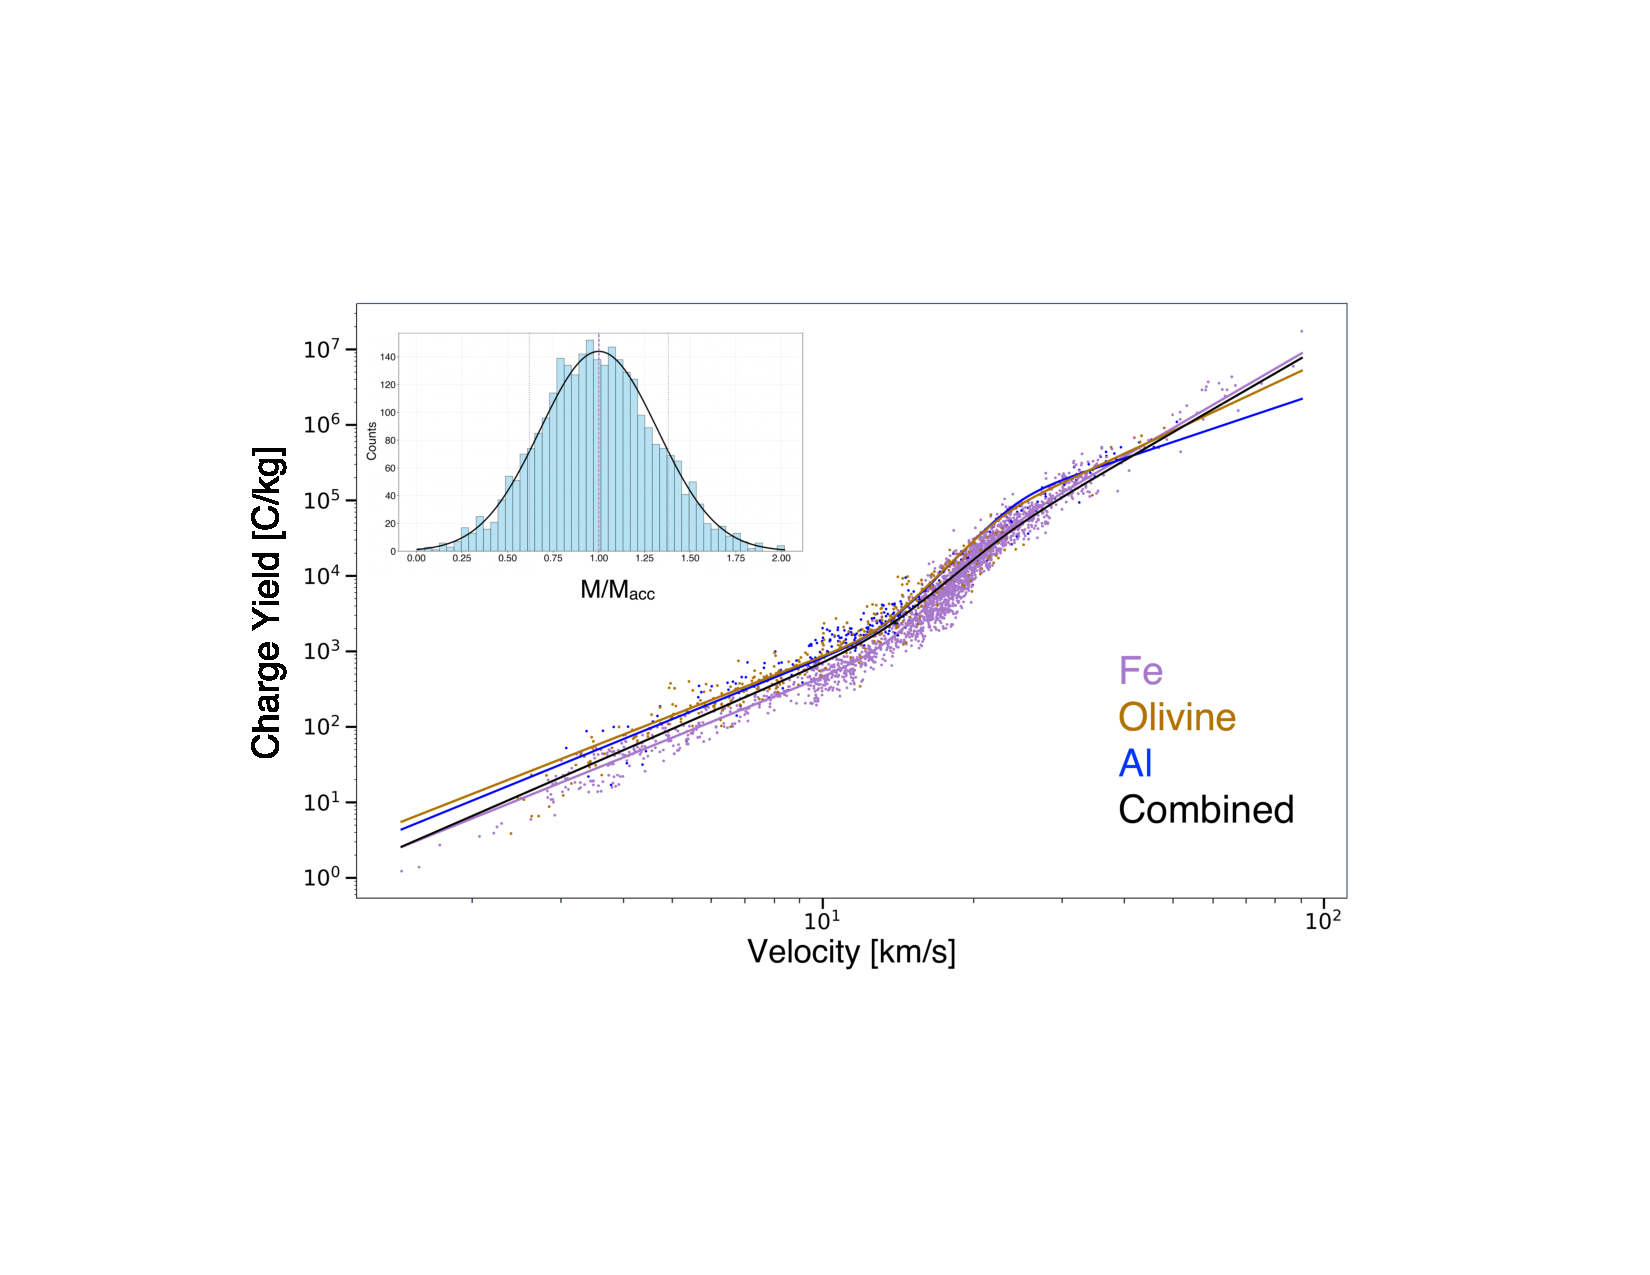
\includegraphics[width=\linewidth]{images/Ethan_yield.pdf}
    \caption{Charge yield for iron (red), aluminum (blue), and olivine (green dots) dust particles.  The insert shows the distribution of the ratio of the dust particle's mass, as calculated from the fit (\autoref{eq:cal}) for all materials combined, over the mass reported by the accelerator.}
    \label{fig:yield}
\end{figure}

The fit parameters for each material used to calibrate IDEX are given below.

\begin{table}[h!]
    \centering
               \renewcommand{\arraystretch}{1}
    \begin{tabular}{|lccccccccc|}


 \rowcolor{darkGrey}    \textcolor{white}{\textbf{}} & \textcolor{white}{\textbf{}} & \textcolor{white}{\textbf{}} &\textcolor{white}{\textbf{}} & \textcolor{white}{\textbf{$QT/M$}} &\textcolor{white}{\textbf{}} & \textcolor{white}{\textbf{}} & \textcolor{white}{\textbf{}} & \textcolor{white}{\textbf{}}&\textcolor{white}{\textbf{}} \\
 \rowcolor{darkGrey}    \textcolor{white}{\textbf{Material}} & \textcolor{white}{{$A$}} & \textcolor{white}{{$a_1$}} &\textcolor{white}{{ $a_2$}} & \textcolor{white}{{$a_3$}} &\textcolor{white}{{$v_b$  [km/s]}} & \textcolor{white}{{$v_c$} [km/s]} & \textcolor{white}{{k}} & \textcolor{white}{{$\sigma$}}&\textcolor{white}{\textbf{$\Delta M_Y$}} \\
        Fe & -0.02 & 2.7 & 6.7 & 3.9 & 13.0 & 23.7 & 11.6& 0.35 & 1.41 \\
   Olivine & 0.32 & 2.6 & 6.7 & 3.1 & 13.0 & 22.8 & 13.9 &0.32 & 1.37 \\
   Al      &0.21  & 2.7 & 6.8 & 2.2 & 13.1 & 24.6 & 12.3 &0.43 & 1.51 \\
Combined   & 0.06 & 2.8  & 5.9 & 4.1 & 13.0 & 22.7  & \ 8.2& 0.40 &1.47\\
     \hline
 \rowcolor{darkGrey}    \textcolor{white}{\textbf{}} & \textcolor{white}{\textbf{}} & \textcolor{white}{\textbf{}} & \textcolor{white}{\textbf{}} & \textcolor{white}{\textbf{{$v$}}} & 
 \textcolor{white}{\textbf{}} & \textcolor{white}{\textbf{}}  & \textcolor{white}{\textbf{}} & \textcolor{white}{\textbf{}}& \textcolor{white}{\textbf{}} \\
  \rowcolor{darkGrey}    \textcolor{white}{\textbf{Material}} & \textcolor{white}{{$A$}} & \textcolor{white}{{$a_1$}} &\textcolor{white}{{ $a_2$}} & \textcolor{white}{{$a_3$}} &\textcolor{white}{{$QT_{\tau}^b$  [$\mu$s]}} & \textcolor{white}{{$QT_{\tau}^c$} [$\mu$s]} & \textcolor{white}{{k}} & \textcolor{white}{\textbf{$\sigma$}}&\textcolor{white}{\textbf{$\Delta v_{QT}$}} \\
 Combined   & 3.6 & -0.2  & -2.0 & 0.38 &\  5.1 & 13.7  & 13.3 & 0.28 & 1.33 \\
     \hline
    \end{tabular}
    \caption{The parameters of the fit of the charge yield as function of the impact speed $Y(v; A, a_1, a_2, a_3, v_b, v_c, k)$ ($top$) and the impact speed as function of the target signal rise time $v(QT_{\tau}; A, a_1, a_2, a_3, v_b, v_c, k)$  ($bottom$) using the same form \autoref{eq:cal}, the standard error $\sigma$ of the Gaussian fitted to the ratio of the fit over the data, and the error factor of the fit  $\Delta M_Y
    \simeq exp(\sqrt{\ln(1 + \sigma^2})$.
    }
\label{tab:params}
\end{table}

In addition to our charge yield curve, our calibration campaign also consisted of developing trends for the target rise time and target to ion grid collection efficiency as a function of speed.

\begin{figure}[H]
    \centering
    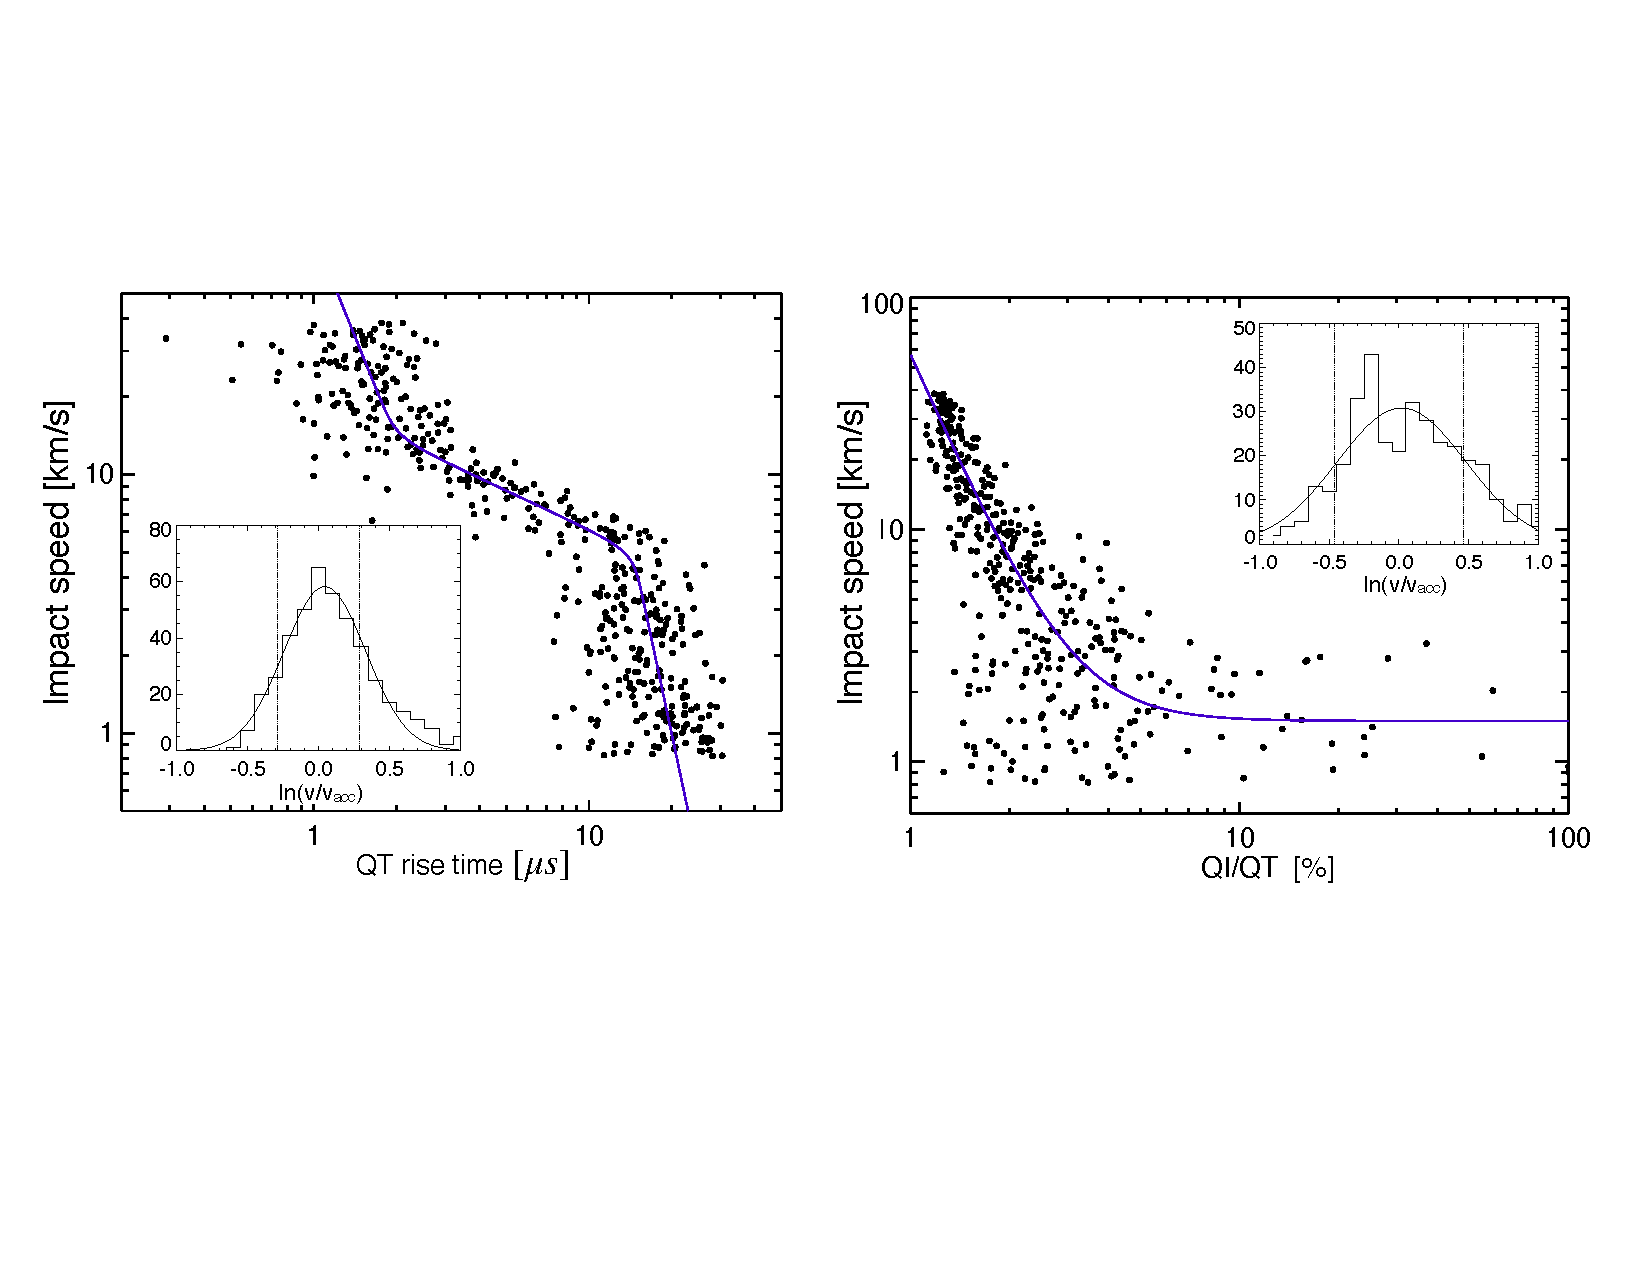
\includegraphics[width=6.5 in]{images/velocity_estimates.pdf}
    \caption{The impact speed of a dust particle as a function of the rise time of  $QT~ (left)$ and the ratio $QI/QT ~(right)$. The inserts show the Gaussian fits to the log of the ratios of the fit over the data, with $\sigma_{QT} \simeq 0.28$ and $\sigma_{QI/QT}  \simeq 0.46$, the error factors ($e^{\sigma}$) are $\Delta v_{QT} \simeq 1.33$  and $\Delta v_{QI/QT} \simeq 1.58$.}
    \label{fig:emtargetyield}
\end{figure}

This calibration curve is the result of both iron and aluminum dust impacts on the IDEX engineering model (EM) using the ground support equipment (GSE) CSAs. It is used at level 2A to provide an estimate for the dust mass with an error factor $\leq$ 2. 

In addition to fitting the target and ion grid signals for impact charge, the TOF mass spectrum's x-axis is converted from time to mass. The algorithm to do so is delineated as follows:

\begin{mdframed}[backgroundcolor=backcolour]{
\begin{enumerate}
    \item Make a vector with all zeros and a length of 8189, same as the TOF length of record: \( t_i \).
    \item Make a vector for masses \( m_i \): 1, 2, 3, 4, …, 200 (200 length, and the elements are the integers 1, 2, 3, …, 200).
    \item Calculate the 200 times (\( T_i \)-s) these masses should show up for a \( T_{\text{off}} = 0 \) and stretch \( A \) (best guess):
          \[
          T_i = T_{\text{off}} + A \sqrt{m_i}
          \]
          and set the closest \( t_i = 1 \) to each of the calculated \( T_i \)-s, leaving the rest as zero.
    \item Calculate the cross-correlation with the original TOF; the maximum will give you the best lag (\( T_{\text{off}} \)) for a given \( A \).
    \item Use an extrema finder to determine the best \( A \). 
\end{enumerate}
} \end{mdframed}

% Once the signal has been fitted, a linear equation is used to convert the amplitude of the fit from pC to V. This linear equation is derived from fits made to the CSAs during EM calibration. An example EM calibration fit is shown in figure~\ref{fig:csacal}.

% \begin{figure}[H]
%     \centering
%     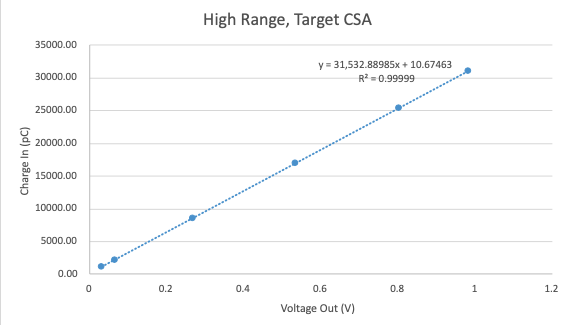
\includegraphics[width=\linewidth]{images/targetcsacal.png}
%     \caption{An example linear fit for the low gain (high range) target CSA.}
%     \label{fig:csacal}
% \end{figure}



\section{Level 2A to 2B Processing}
For the level 2B  data product, a spectrogram of the number of dust hits as a function of both mass and time will be generated. The simulation data depicted in \autoref{fig:isdpop} can be used to generate example files for these. The dataset records the count rate of detected dust particle impacts as a function of several key parameters: 


\begin{itemize}
    \item \textbf{Time of Impact} ($t$) - The timestamp of each dust detection event.
    \item \textbf{Spin Phase} ($\phi$) - The spacecraft spin phase at the time of detection. This is given in quadrants (0, 90, 180, 270).
    \item \textbf{Mass or Charge} ($m/q$) - The estimated mass or charge of the detected dust particle.
    \item \textbf{Count rate} ($N/\Delta t_{acc}$) - The number of detected dust particles in a given bin per accumulation time $t_{acc}$, where the accumulation time is the width of the time bin subtracted by any dead times.
\end{itemize}

\noindent\textbf{Science Acquisition Timestamp Extraction}

The Science Data Center (SDC) uses IDEX event telemetry to determine periods of science data collection. The IDEX instrument generates event files containing operational state information that are ingested and decommutated daily by the SDC.

The Level~2B (L2B) processing pipeline is triggered monthly and includes all event CDF files from the preceding month plus a two-week buffer period. This span ensures complete coverage for determining instrument operational states across processing boundaries.

The SDC processes event datasets through the following steps:
\begin{enumerate}
  \item \textbf{Data Preparation:} Event data are sorted chronologically by epoch timestamp, and duplicate entries are removed to ensure temporal consistency.

  \item \textbf{State Change Event Identification:} Science state-change events are identified by filtering for event packets with identifier \texttt{SCI\_STE} (Science State Event).

  \item \textbf{Parameter Reconstruction:} For each state-change event, two 16-bit parameter values are reconstructed by combining pairs of 8-bit telemetry parameters:
  \begin{itemize}
    \item \texttt{val1 = (el1par\_evtpkt << 8) | el2par\_evtpkt}
    \item \texttt{val2 = (el3par\_evtpkt << 8) | el4par\_evtpkt}
  \end{itemize}

  \item \textbf{Acquisition State Classification:} State transitions are classified based on parameter value combinations:
  \begin{itemize}
    \item \emph{Science Start:} \texttt{val1=ACQSETUP} and \texttt{val2=ACQ} indicate transition to active data acquisition.
    \item \emph{Science Stop:} \texttt{val1=ACQ} and \texttt{val2=CHILL} indicate transition to idle/standby state.
  \end{itemize}
\end{enumerate}

The charge and mass estimates are placed into 10 bins for the Level 2B IDEX data product. These bins and their ranges are given in table \ref{tab:charge_mass_bins}.

% Requires in preamble (once): \usepackage[table]{xcolor} \definecolor{darkGrey}{RGB}{77,77,77}

\begin{table}[h!]
\centering
\renewcommand{\arraystretch}{1.9}
\setlength{\tabcolsep}{8pt}
\begin{tabular}{|c|c|c|}
\hline
\rowcolor{darkGrey}
\textcolor{white}{\textbf{Bin}} &
\textcolor{white}{\textbf{Mass range [kg]}} &
\textcolor{white}{\textbf{Charge range [pC]}} \\
\hline
1  & $6.31\times10^{-17}$--$1.00\times10^{-16}$ & $1.00\times10^{-1}$--$3.16\times10^{-1}$ \\
2  & $1.00\times10^{-16}$--$1.58\times10^{-16}$ & $3.16\times10^{-1}$--$1.00\times10^{0}$ \\
3  & $1.58\times10^{-16}$--$2.51\times10^{-16}$ & $1.00\times10^{0}$--$3.16\times10^{0}$ \\
4  & $2.51\times10^{-16}$--$3.98\times10^{-16}$ & $3.16\times10^{0}$--$1.00\times10^{1}$ \\
5  & $3.98\times10^{-16}$--$6.31\times10^{-16}$ & $1.00\times10^{1}$--$3.16\times10^{1}$ \\
6  & $6.31\times10^{-16}$--$1.00\times10^{-15}$ & $3.16\times10^{1}$--$1.00\times10^{2}$ \\
7  & $1.00\times10^{-15}$--$1.58\times10^{-15}$ & $1.00\times10^{2}$--$3.16\times10^{2}$ \\
8  & $1.58\times10^{-15}$--$2.51\times10^{-15}$ & $3.16\times10^{2}$--$1.00\times10^{3}$ \\
9  & $2.51\times10^{-15}$--$3.98\times10^{-15}$ & $1.00\times10^{3}$--$3.16\times10^{3}$ \\
10 & $3.98\times10^{-15}$--$1.00\times10^{-14}$ & $3.16\times10^{3}$--$1.00\times10^{4}$ \\
\hline
\end{tabular}
\caption{Bin definitions for mass and charge used for IDEX L2B data products.}
\label{tab:charge_mass_bins}
\end{table}

For the edge case that a mass or charge value is below the value 

The following table presents a sample of the Level 2B data product. The values represent binned counts of detected dust particles:






\begin{table}[h]
    \centering
    \caption{\textbf{Daily Binned Dust Hit Counts as a Function of Time, Spin Phase, and Mass/Charge}}
    \label{tab:dust_counts}
    \renewcommand{\arraystretch}{1.3}
    \setlength{\arrayrulewidth}{1.2pt}
    \begin{tabular}{c c c c}
        \hline\hline
        \textbf{Date (UTC)} & \textbf{Spin Phase (deg)} & \textbf{Mass/Charge ($\si{kg}$ or $\si{C}$)} & \textbf{Rate ($s^{-1}$)} \\
        \hline\hline
        2027-02-18 & \textbf{0}  & \textbf{$1.2 \times 10^{-15}$}  & \textbf{32}  \\
        2027-02-19 & \textbf{90} & \textbf{$3.5 \times 10^{-16}$}  & \textbf{60} \\
        2027-02-20 & \textbf{180} & \textbf{$2.51 \times 10^{-15}$}  & \textbf{25}  \\
        2027-02-21 & \textbf{270} & \textbf{$4.8 \times 10^{-16}$}  & \textbf{48} \\
        \hline\hline
    \end{tabular}
\end{table}

\textbf{Please note that: }
\begin{itemize}
    \item Times are given in Coordinated Universal Time (UTC).
    \item Spin phase is defined relative to an inertial (despun) reference frame.
    \item Mass and charge values are estimated using calibration data.
\end{itemize}

\section{Level 2A to 2C Processing}

Generate pointing sets from level 2A. All events will be dust, so pointing sets follow directly. Count rates are encoded in the pointing sets. We want RTN for IDPs, EJ2000 for ISD. A time-ordered list of time, boresight vector for every impact. We will also need accumulation times. Disregard events that are flagged as SW triggers.

For the level 2C data products, maps of flux, rates and composition will be generated, using the IBEX ENA maps as reference. An example of a historical dust map for the interstellar dust is shown in \autoref{fig:isdmap}.


\begin{figure}[H]
    \centering
    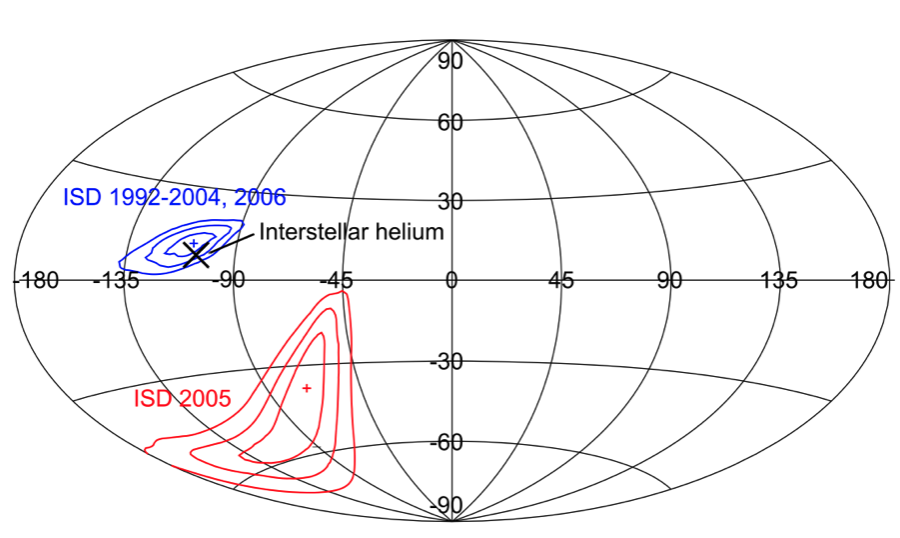
\includegraphics[width=6.5 in]{images/isd_deflection_map.png}
    \caption{Map of the two different deflections of interstellar dust measured by Cassini's CDA and Ulysses from the nominal interstellar helium flow direction into the solar system. }
    \label{fig:isdmap}
\end{figure}.

These maps will require defining \textbf{pointing sets}, which contain the data binned by instrument boresight vector. For IDEX maps, each dust impact is assumed to come directly from the boresight direction (neglecting the 50-degree field-of-view).

Typical data for a 2 year mission are shown in figure \ref{fig:mappedcounts}. The y and x axes represent the EJ2000 latitude and longitude, respectively. The incoming ISD direction is apparent from the enhancement at (8, -118).

\begin{figure}[h!]
    \centering
    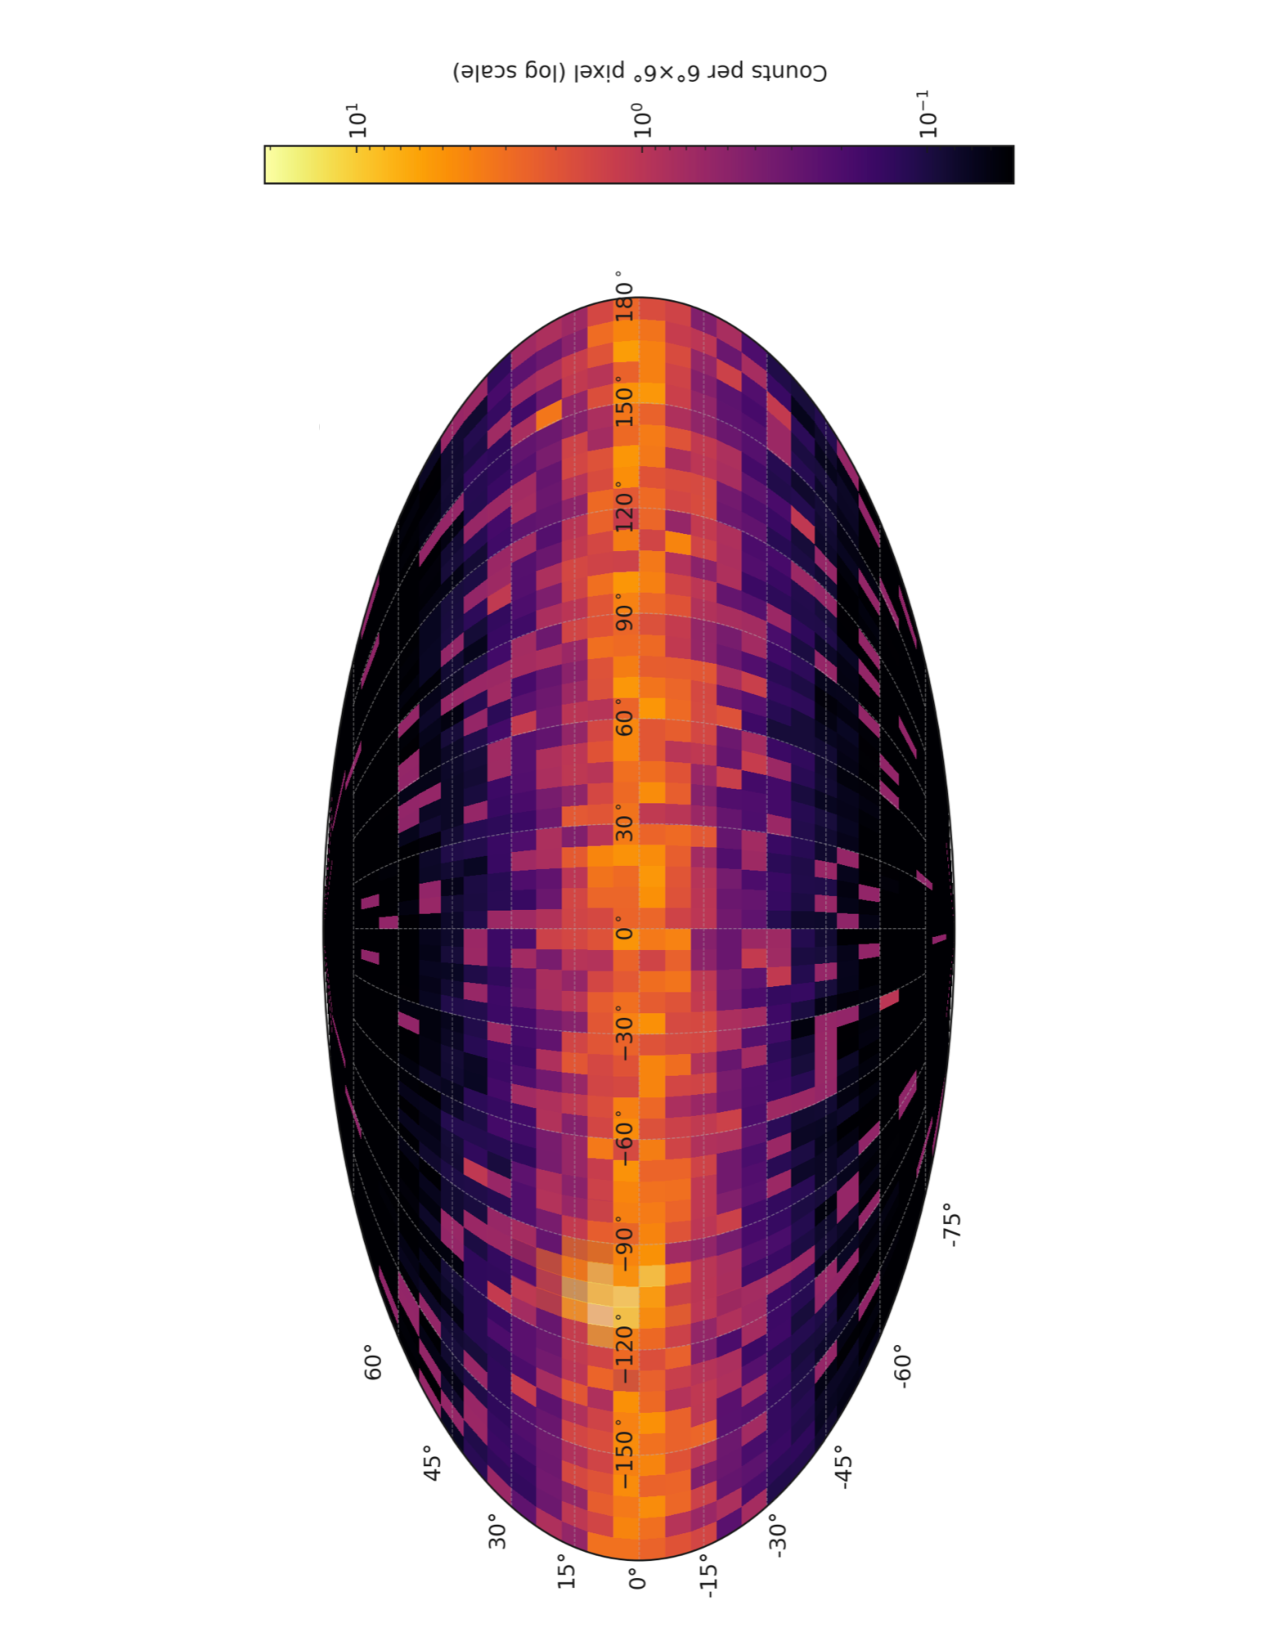
\includegraphics[angle=270, width=0.8\linewidth]{images/Mollweide_Zodiacal_dust_sky_map.pdf}
    \caption{Total dust counts per 6 x 6 degree pixels in latitude and longitude in EJ2000. This is assuming a dust instrument mounted to a spacecraft at 1 AU, such as IDEX. These maps will be used for direct comparison of the COMIT model's results with IMAP results. In addition to total dust counts, they will be generated for a given impact charge, mass and dust composition type (silicate, organic, etc.) for further comparison with IDEX.}
    \label{fig:mappedcounts}
\end{figure}

% \chapter{Level 0 to 1}

The initial step in the IDEX data pipeline is to convert level 0 data to level 1. This entails two steps; namely,

\begin{enumerate}
\item \textbf{Level 0 to 1A}: Converting CCSDS packets to Time tagged event data, coincident, target and ion grid waveforms, and time-of-flight spectra in data number (DN)
\item \textbf{Level 1A to 1B}: Taking the 1A data and converting the data number spectra to voltage spectra.
\end{enumerate}

\subsection{Jamey Meeting (1/14/22)}
\begin{itemize}
    \item Python “0 to 1” code can be handed over to the SOC instead of pseudo code
\item Packetcrushing code will be useful for calibration
\item CCSDS decommutation in Python may be available
\item Make sure APID’s are in order for the CCSDS packets (FPGA testing) - reach out to Wendy \textbf{Completed that same day}
\item Get the definitions, and try to write it with the synthetic spectra and test it
\item 1: dN, 2: Volts, 3: ion mass
\item Make sure we interface with the mapping groups (ENA pipeline is not so different than our instrument)
\end{itemize}


The contents of each APID are further described below.  All IDEX packets are \textbf{32-bit aligned, start with a CCSDS header, and end with a 2-byte CRC} (see IICD JPL D-55881 for details).  A 32-bit Unified Message Structure header appears before the CCSDS header, but is expected to be removed by the spacecraft before it get to the ground.
\newline
\newline
In general, science data is organized onboard by the \textbf{accountability identifier (AID)}.  The AID is assigned when the data is acquired, and is used to access the data afterwards.  The AID cannot be changed, and duplicate AIDs are not permitted.  Each dataset is composed of one or more \textbf{“events”}, which is a collection of data collected when the instrument triggers, usually representing a dust particle impact.  Each event is given a unique “event number” by the FPGA, so that every event collected by IDEX can be uniquely identified by the combination of AID and event number.  

SUDA Event data is composed of seven distinct parts:
\begin{enumerate}
\item	Time of Flight (TOF) waveform data on the high-gain (HG) channel, sampled at 250 megasamples per second (Msps) with 10 bit resolution
\item	TOF waveform data on the mid-gain (MG) channel, sampled at 250 Msps with 10 bit resolution
\item	TOF waveform data on the low-gain (LG) channel, sampled at 250 Msps with 10 bit resolution
\item	Velocity (Qv) grid charge sensitive amplifier (CSA) waveform data, sampled at 3.75 Msps with 12 bit resolution
\item	Ion (Qi) grid CSA waveform data, sampled at 3.75 Msps with 12 bit resolution
\item	Target (Qt) CSA waveform data, sampled at 3.75 Msps with 12 bit resolution
\item	FPGA Pre-pended metadata header containing IDEX’s configuration and status at the time of the trigger, recorded by the FPGA
\end{enumerate}


\section{Heritage Processing}
This section describes the development of Python code to convert level 0 data to level 1A. The code described below can be found in the pipeline dropbox under "/python/Level 0$\rightarrow$1/Python Packet Crushing"

\begin{figure}[H]
    \centering
    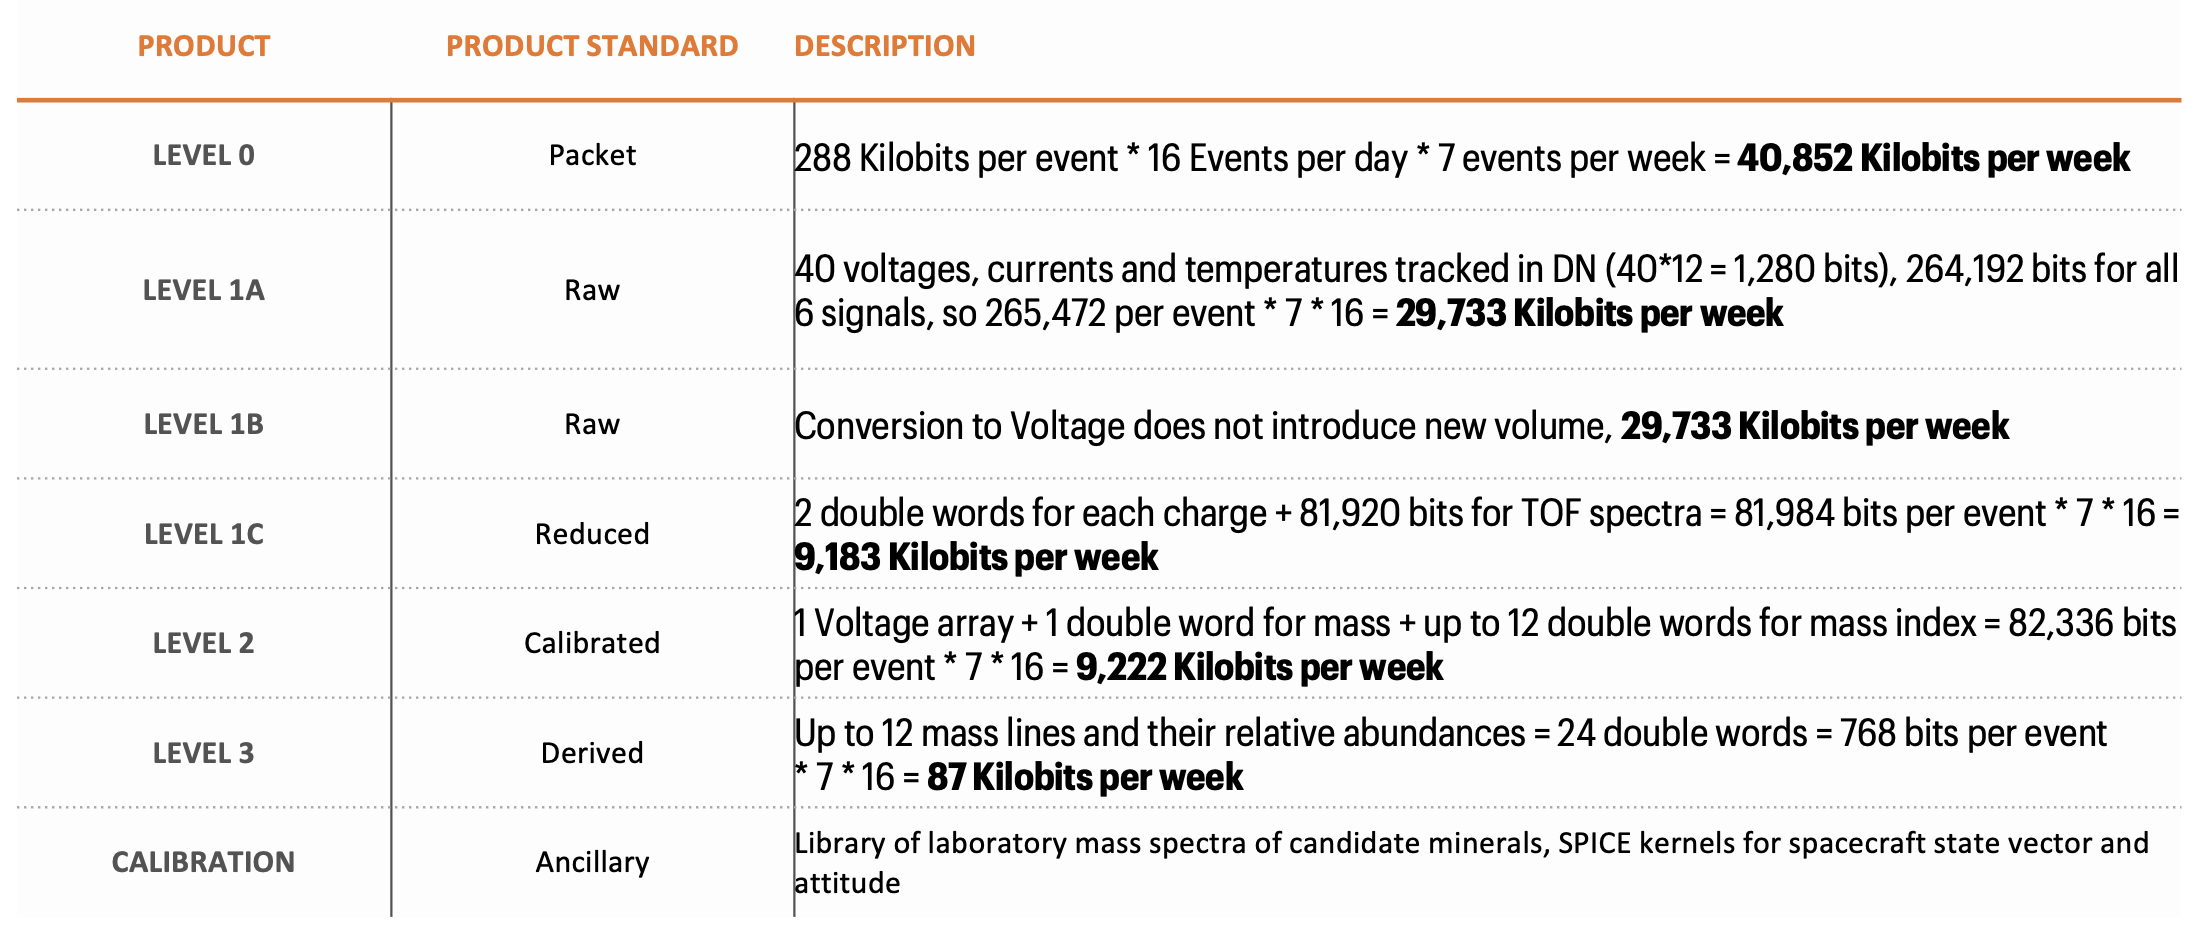
\includegraphics[width=\linewidth]{images/DataVolume.png}
    \caption{An outline of the data volume by product level. This is based on FPGA buffers and packetizing overhead.}
    \label{fig:datavolume}
\end{figure}

\begin{figure}[H]
    \centering
    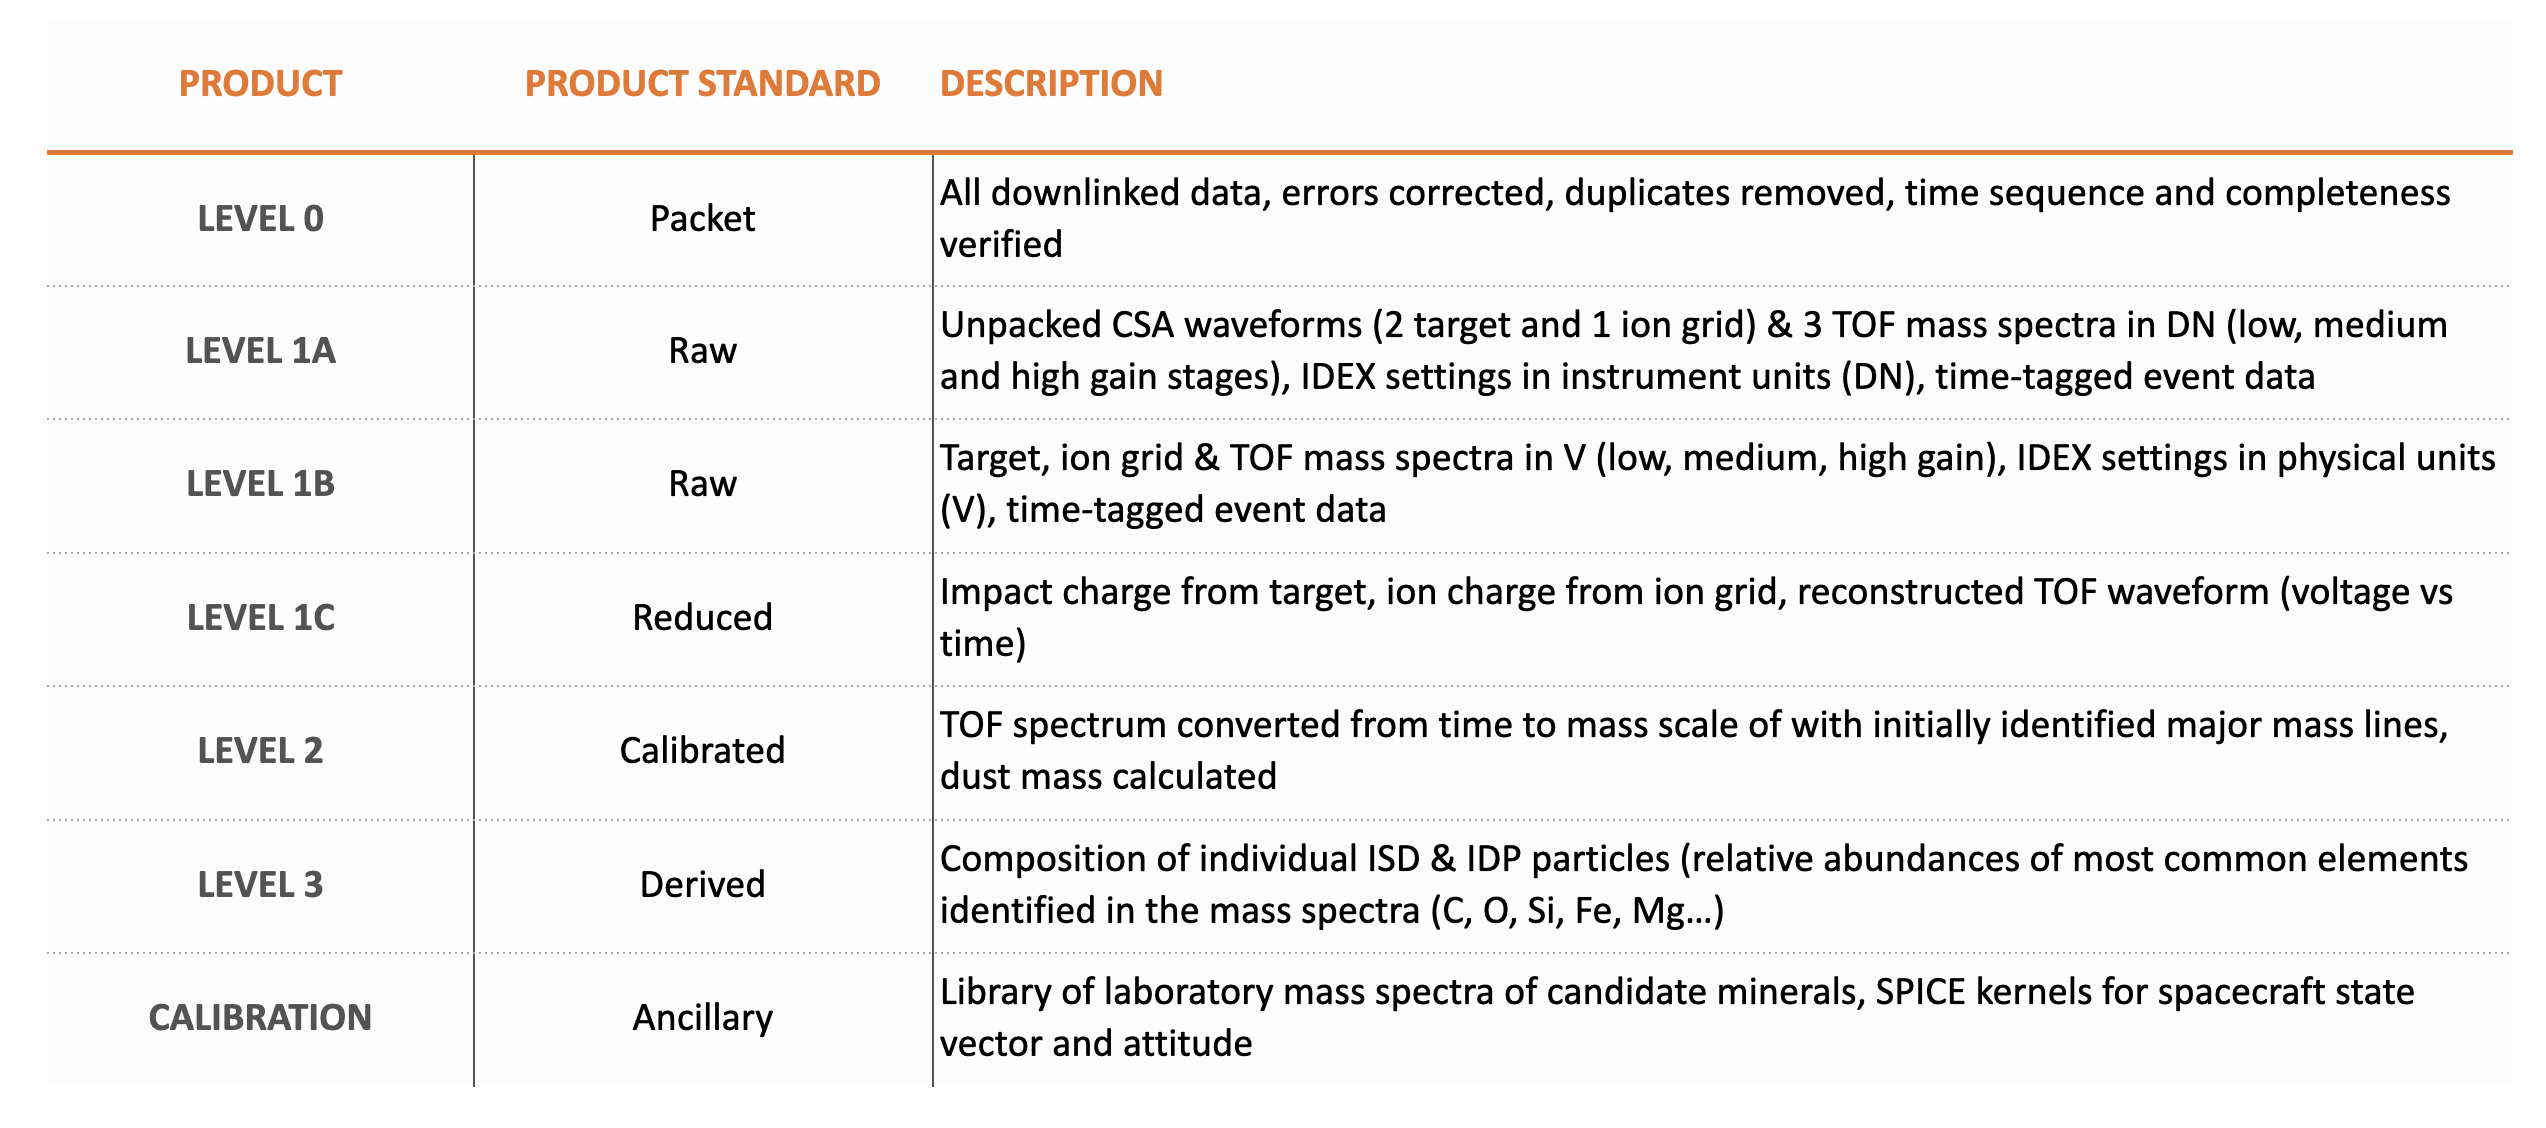
\includegraphics[width=\linewidth]{images/pipeline.png}
    \caption{An outline of each data product level containing the corresponding data type and description.}
    \label{fig:pipeline}
\end{figure}





\begin{figure}[H]
    \centering
    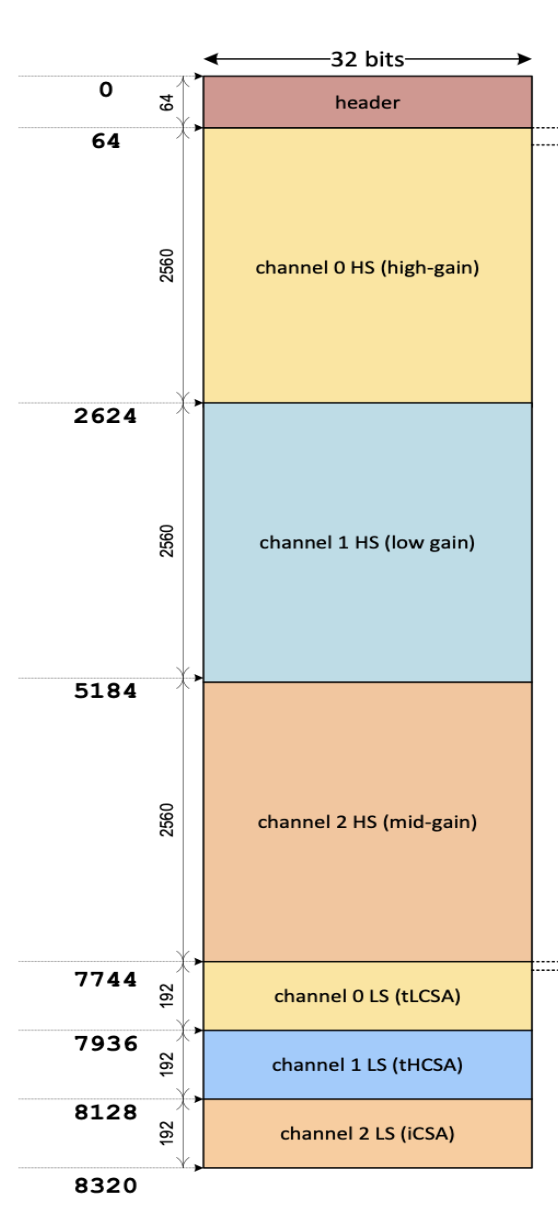
\includegraphics[width=\linewidth]{images/Waveform_Structure.png}
    \caption{An outline of IDEX's channels, with their bit length. Only specific packets contain waveforms.}
    \label{fig:db}
\end{figure}
\subsection{Hydra Packets:}
We chose to start by reading in the Hydra science packets from their raw .xml files. These files are similar to html, minus the prewritten tags. They follow the anatomy delineated in the figure below:


\begin{figure}[H]
    \centering
    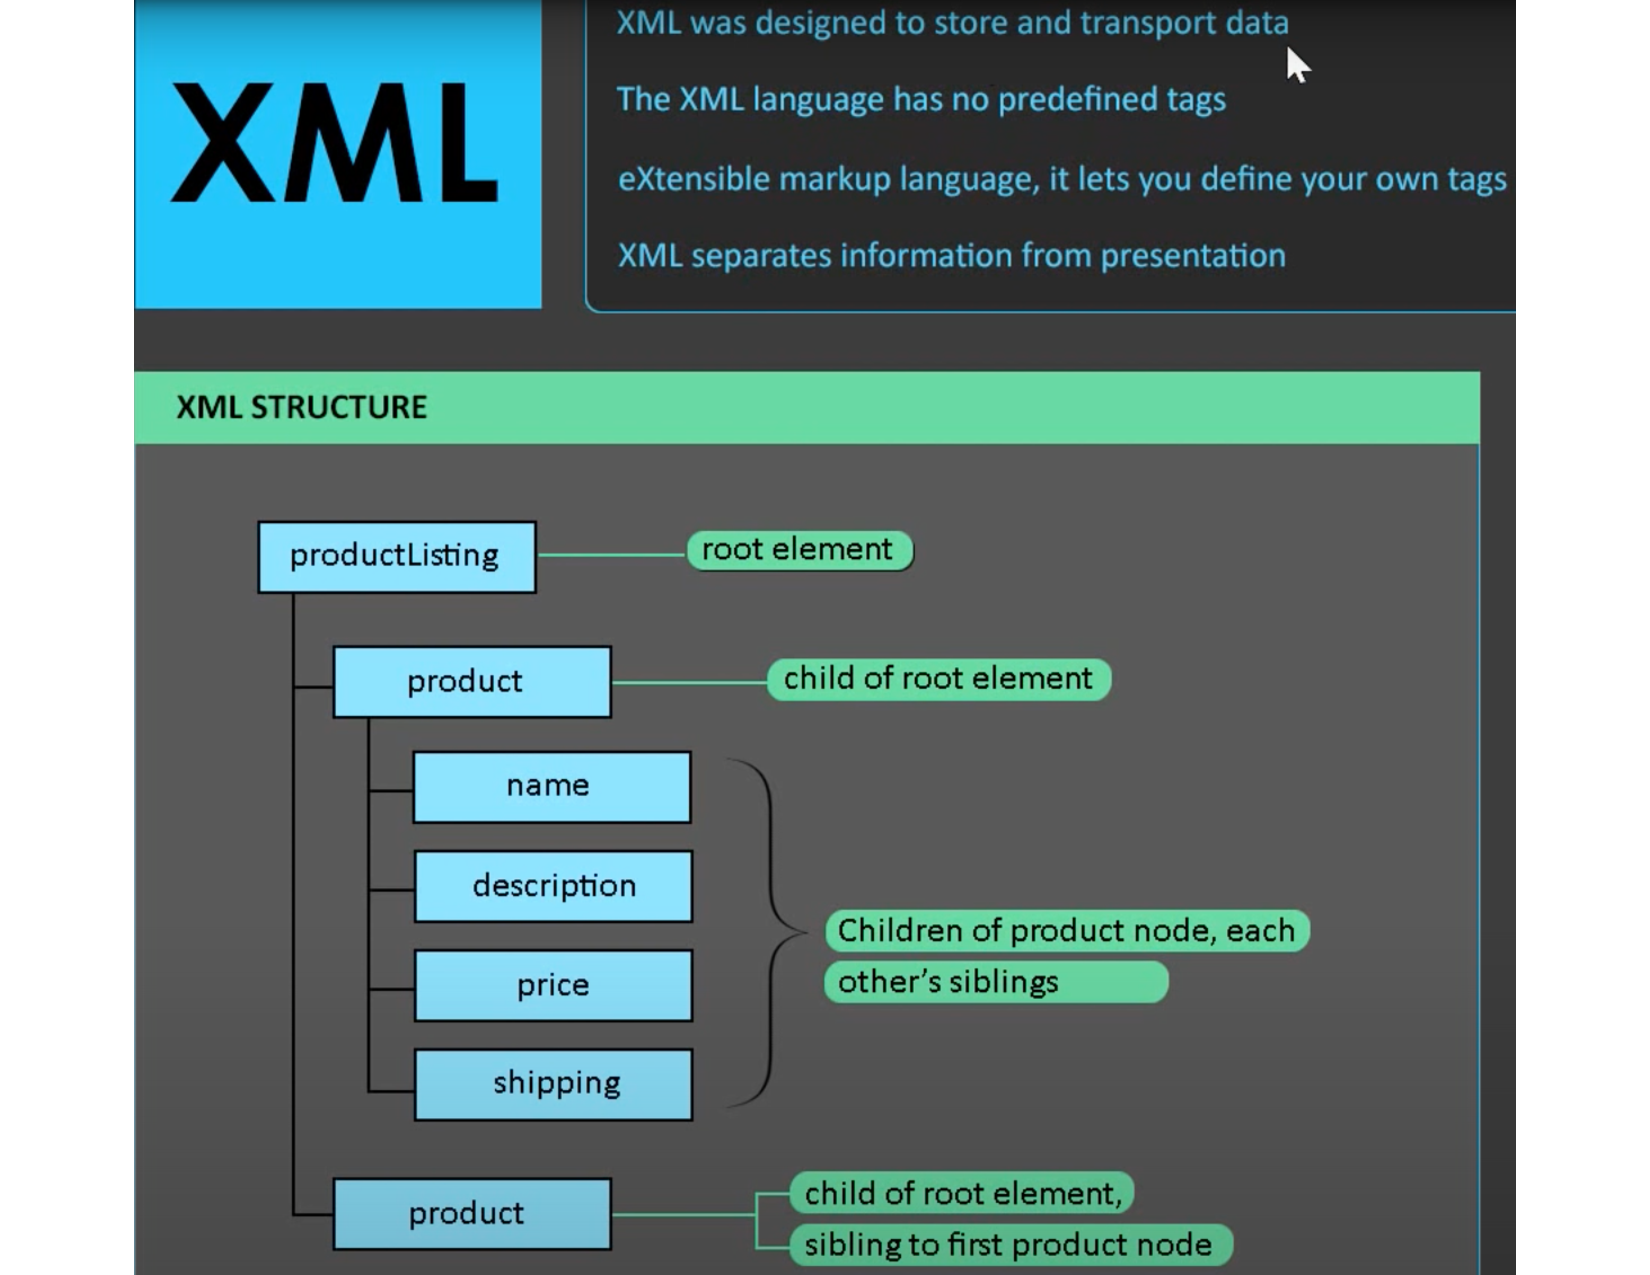
\includegraphics[width=12cm]{images/xml.pdf}
    \caption{Anatomy of an xml document along with some general notes. }
    \label{fig:massline-byloc}
\end{figure}


\section{Next steps:}
\begin{enumerate}
\item Focus on ion calibration part of the packet
\item Once we get level 0, the TOF channel is this large with this many units, etc. $\rightarrow$ Data volume figure \ref{fig:datavolume}
\item Give dtypes and volumes from SDC document $\rightarrow$ White paper
\item Describe the APIDS we've inherited from SUDA $\rightarrow$ Outlined, finish translating white paper
\item Describe hierarchical decision tree $\rightarrow$ Text description from greg, make a diagram
\item Provide the calibration curve in terms of the fits (The final calibration) $\rightarrow$ Heritage SUDA and LDEX curves available

\end{enumerate}


\setcounter{chapter}{0}
\renewcommand{\chaptername}{Appendix}
\renewcommand{\thechapter}{\Alph{chapter}}

\chapter{LASP Packets}\label{lasppackets}
The \textbf{generator} method from the \textbf{parser.py} script in LASP Packets.

\pythonstyle
\begin{lstlisting}[language=Python,breaklines]
def generator(self, binary_data: bitstring.ConstBitStream, parse_bad_pkts: bool = True, skip_header_bits: int = 0, root_container_name="CCSDSPacket", ccsds_headers_only: bool = False, yield_unrecognized_packet_errors: bool = False, show_progress: bool = False):
    """Create and return a Packet generator.
    Creating a generator object to return allows the user to create many generators from a single Parser and reduces memory usage.
    ...
\end{lstlisting}

\chapter{IDEX/SUDA Combined XTCE Definition}\label{xtce}
The first 100 lines of the combined IDEX/SUDA XTCE definition are shown below.

\IfFileExists{suda_combined_definition.xml}{%
  \lstinputlisting[basicstyle=\ttfamily\scriptsize,breaklines=true,language=XML,firstline=1,lastline=98]{suda_combined_definition.xml}%
}{%
  \begin{mdframed}
    \emph{File \texttt{suda\_combined\_definition.xml} not found. Place it in the project root to include it.}
  \end{mdframed}
}

\end{document}
